\chapter{Object Reconstruction and Identification}\label{obj_reco_id}

\section{Primary Vertices}

In general, many primary vertices are reconstructed in an event beacuse of the pileup contributions. In order to identify the vertex related with the main proton-proton collision in the analized event,  we required that:

\begin{itemize}
\item
Number of degrees of freedom:  $n_{\text{dof}} >$ 4
\item
longitudinal coordinate: $z_{0} <$ 24 mm
\item
Transverse position: $d_{0}<$ 2 mm 
\item
Vertex fit variable: $\chi^{2} \neq$ 0
\end{itemize}

If more than one vertex pass the previous conditions, we choose the one with the highest sum of transverse momenta $\sum \pt^{2}$ of the \emph{tracks} associated to it. 
Due to disagreements in the number of primary vertices distribution  between the MC samples and data a reweight procedure was implemented assuming a total inelastic cross section of $\sigma = 69 000 \mu$b. Figure \ref{fig:nv} (Left) shows the comparison for the PU in data and MC (Right) the distribution of the number of primary vertices after apply the reweight procedure. 

\begin{figure}[!ht]
\caption{Left: Comparison between the PU profile in data (blue) and the Poisson density function in MC (green). Right: Number of primary vertices distribution after the reweight procedure in events that pass the final analysis selection.}
\begin{tabular}{cc}
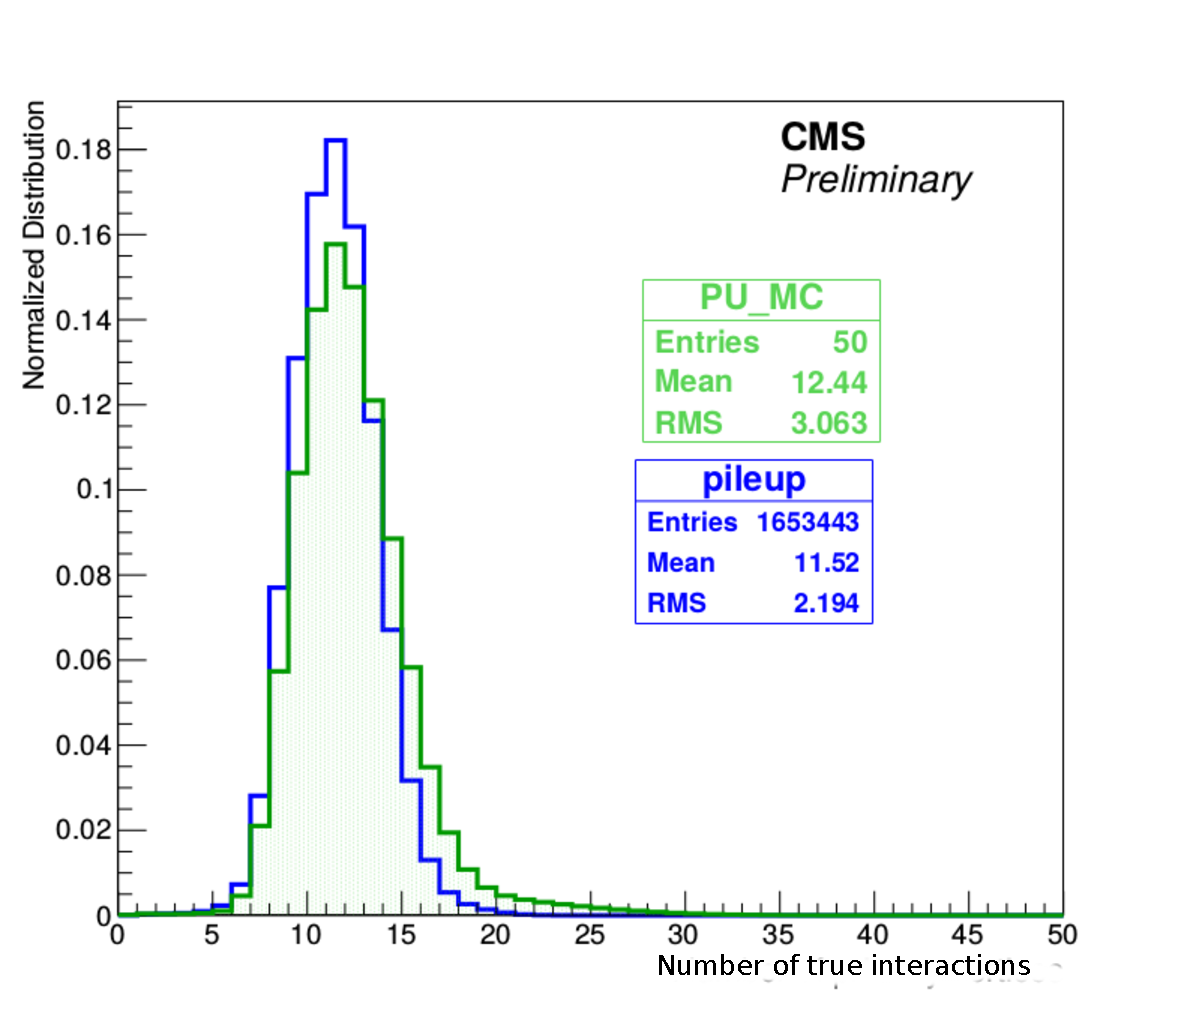
\includegraphics[width=250pt]{figures/Objects/PV.pdf}&
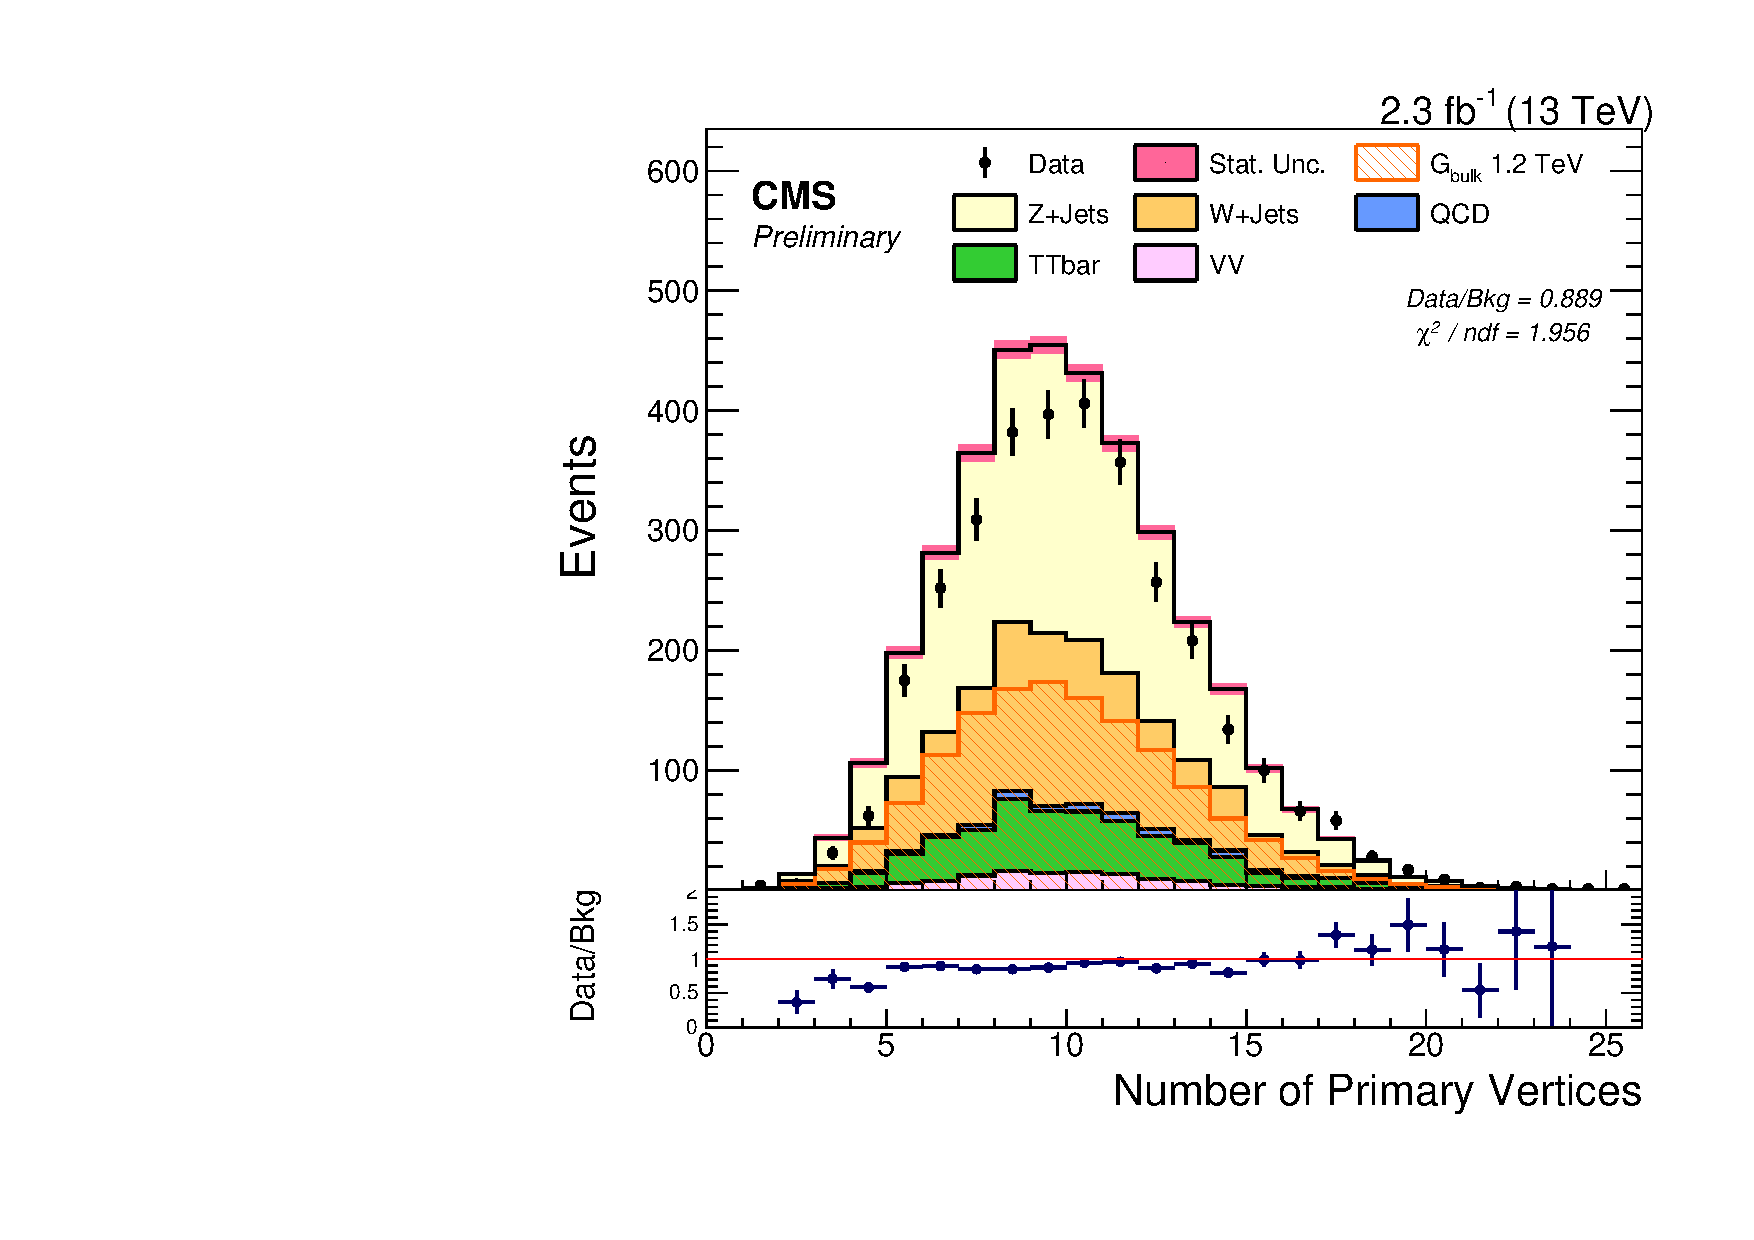
\includegraphics[width=210pt]{figuresARC/CONTROLPLOTS/can_h_nVtx.pdf}\\
\end{tabular}
\label{fig:nv}
\end{figure}

\section{Missing Transverse Energy}\label{met}

The raw missing transverse energy vector is computed as the negative vector sum of the transverse momenta of all particles reconstructed in the event, with magnitude denoted by $\MET$. Corrections to the momenta of jets reconstructed in the event are further propagated to the $\MET$ (Type-1 corrections) \cite{CMS:2016ljj}. Figure \ref{fig:MET} show a comparison between the raw PF $\MET$ and the Type-1 PF $\MET$.

\begin{figure}[!ht]
\caption{Comparison between Raw PF $\MET$ and Type-1 PF $\MET$ corresponding to a signal sample of 1 TeV.}
\begin{center}
  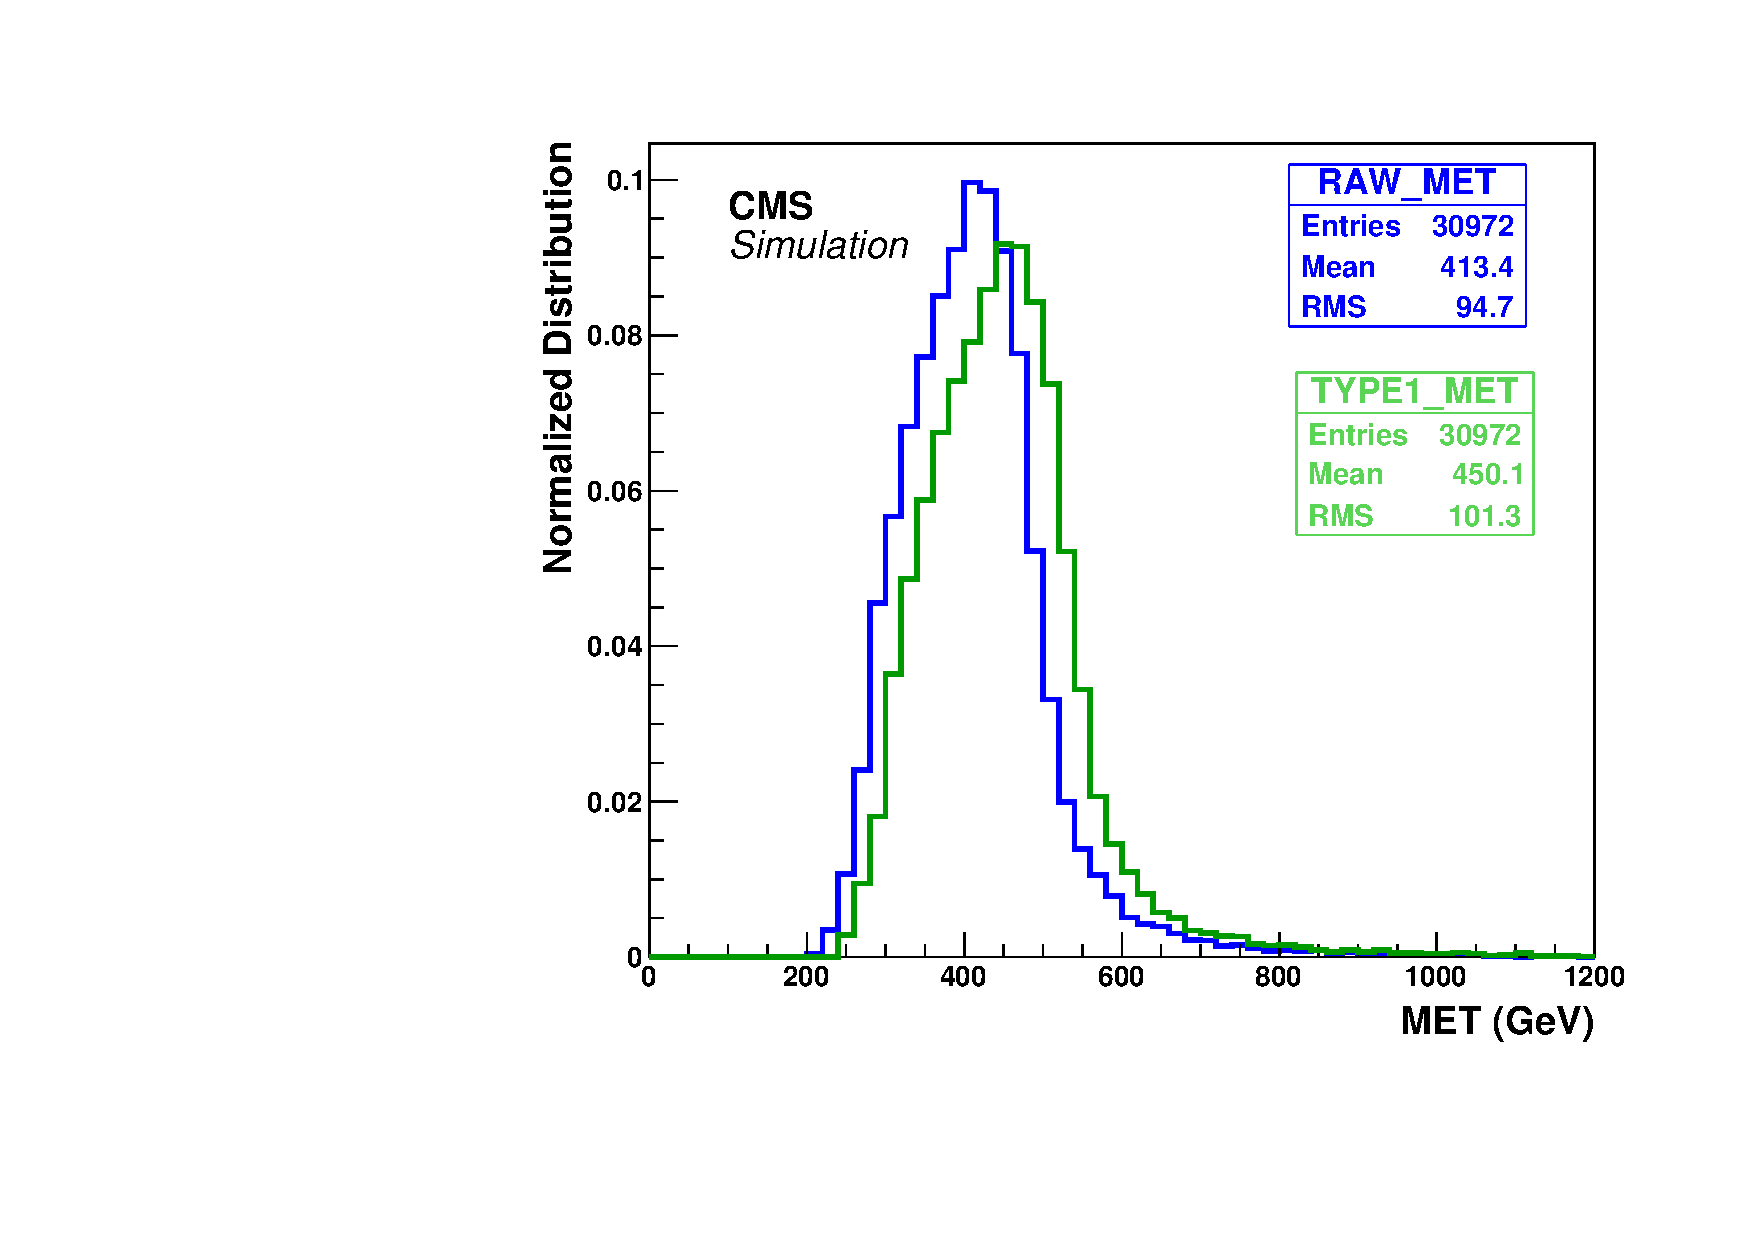
\includegraphics[width=280pt]{figures/Objects/metcomparison.pdf}
\end{center}
\label{fig:MET}
\end{figure}

A set of dedicated quality filters are applied in data and simulation to remove events with a large misreconstructed $\MET$ originated from detector noise and beam backgrounds \cite{CMS:2016ljj}:

\begin{itemize}
\item
HBHENoiseFilter
\item
HBHENoiseIsoFilter
\item
CSCTightHalo2015Filter
\item
EcalDeadCellTriggerPrimitiveFilter
\item
goodVertices
\item
eeBadScFilter
\end{itemize}

\begin{figure}[!ht]
\caption{HBHENoiseFilter efficiency vs AK8 jet $\pt$ in simulation for a signal sample of 1 TeV.}
\begin{center}
  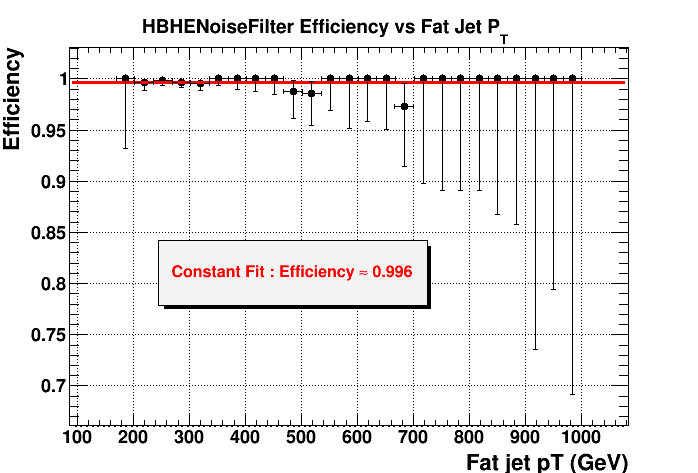
\includegraphics[width=280pt]{Chapter5_plots/effFilter.png}
\end{center}
\label{fig:METfilter}
\end{figure}

Figure \ref{fig:METfilter} shows the efficiency for the events that pass the HBHENoiseFilter for signal sample of 1 TeV. Events containing a minimum $\MET$ of 250 GeV are required in the analysis in order to settle in the plateau of the trigger turn-on curve (Fig. \ref{fig:TriggerEff1}). Further corrections are applied to the $\MET$ in the V+jets simulated samples, based on the hadronic recoil information derived from Z+jets ($Z\rightarrow \ell \ell$)  events in data and simulation (Recoil Correction).

\subsection{Recoil Correction}

We use a data-driven method to model the V boson recoil (response and resolution) in order to improve the description of the missing energy in  V+jets MC events. The term ``recoil'' here means the hadronic activity that balances the $\pt$ of the boson.  To derive the recoil correction we use a Z +jets ($Z \to \mu \mu$ ) process in data and simultion, fitting the response and resolution of the recoil as a function of Z $\pt$. The advantage of using the $Z$+jets process is that the Z boson can be selected without significant background and the $\pt$ can be accurately reconstructed in data from the two final state leptons. The transverse recoil vector is defined as:
\begin{eqnarray}
\vec{u}_{\mathrm{T}} = -\vec{\MET}-\Sigma_{i} \vec{\ell}_{i}
\end{eqnarray}
where $\vec{\ell}_{i}$ is the momentum of the lepton in which the Z decays. Figure \ref{fig:recoil01} shows the kinematics of the process in the transverse plane. The method parametrize the recoil in the parellel and perpendicular directions of the boson $\pt$, fitting these variables with a double gaussian model in different bins of the Z $\pt$. From the fits it can extract the mean an the $\sigma$ of the gaussians, using different polynomial functions to fit these values and extract the response and resolution curves. After this process some scale factors are derived and applied to the  V+jets simulated samples. Complementary information about the recoil method is reported in the Appendix \ref{appendix:ApendiceB}.

\begin{figure}[!ht]
\caption{$Z\rightarrow \ell \ell$ event kinematics in the transverse plane. The transverse recoil vector $\vec{u}_{\mathrm{T}}$ is split into parallel and perpendicular components to the direction of the boson $\pt$. }
\begin{center}
  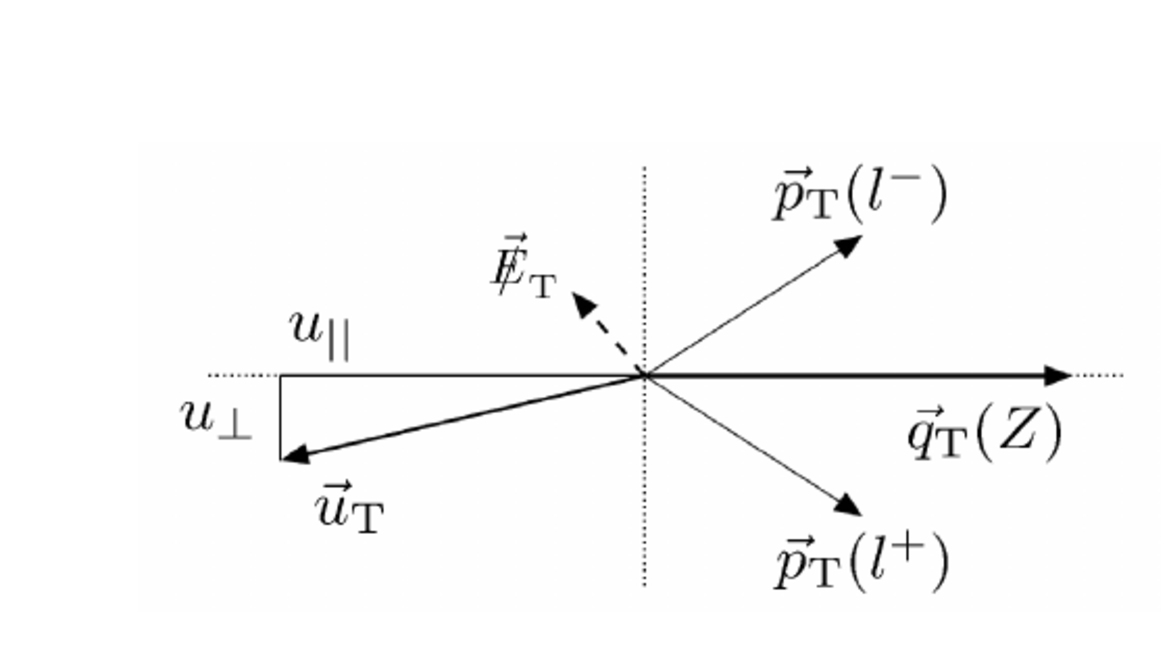
\includegraphics[width=280pt]{Chapter5_plots/recoil.pdf}
\end{center}
\caption*{Source: CMS Collaboration, “Performance of missing energy reconstruction in 13
TeV pp collision data using the CMS detector”, CMS-PAS-JME-16-004, 2016.}
\label{fig:recoil01}
\end{figure}

Figure \ref{fig:METrecoil} shows the transverse missing energy distribution before and after apply the recoil corrections.

\begin{figure}[!ht]
\caption{$\MET$ distribution before and after apply the recoil correction for W +jets and Z + jets samples.}
\begin{tabular}{cc}
  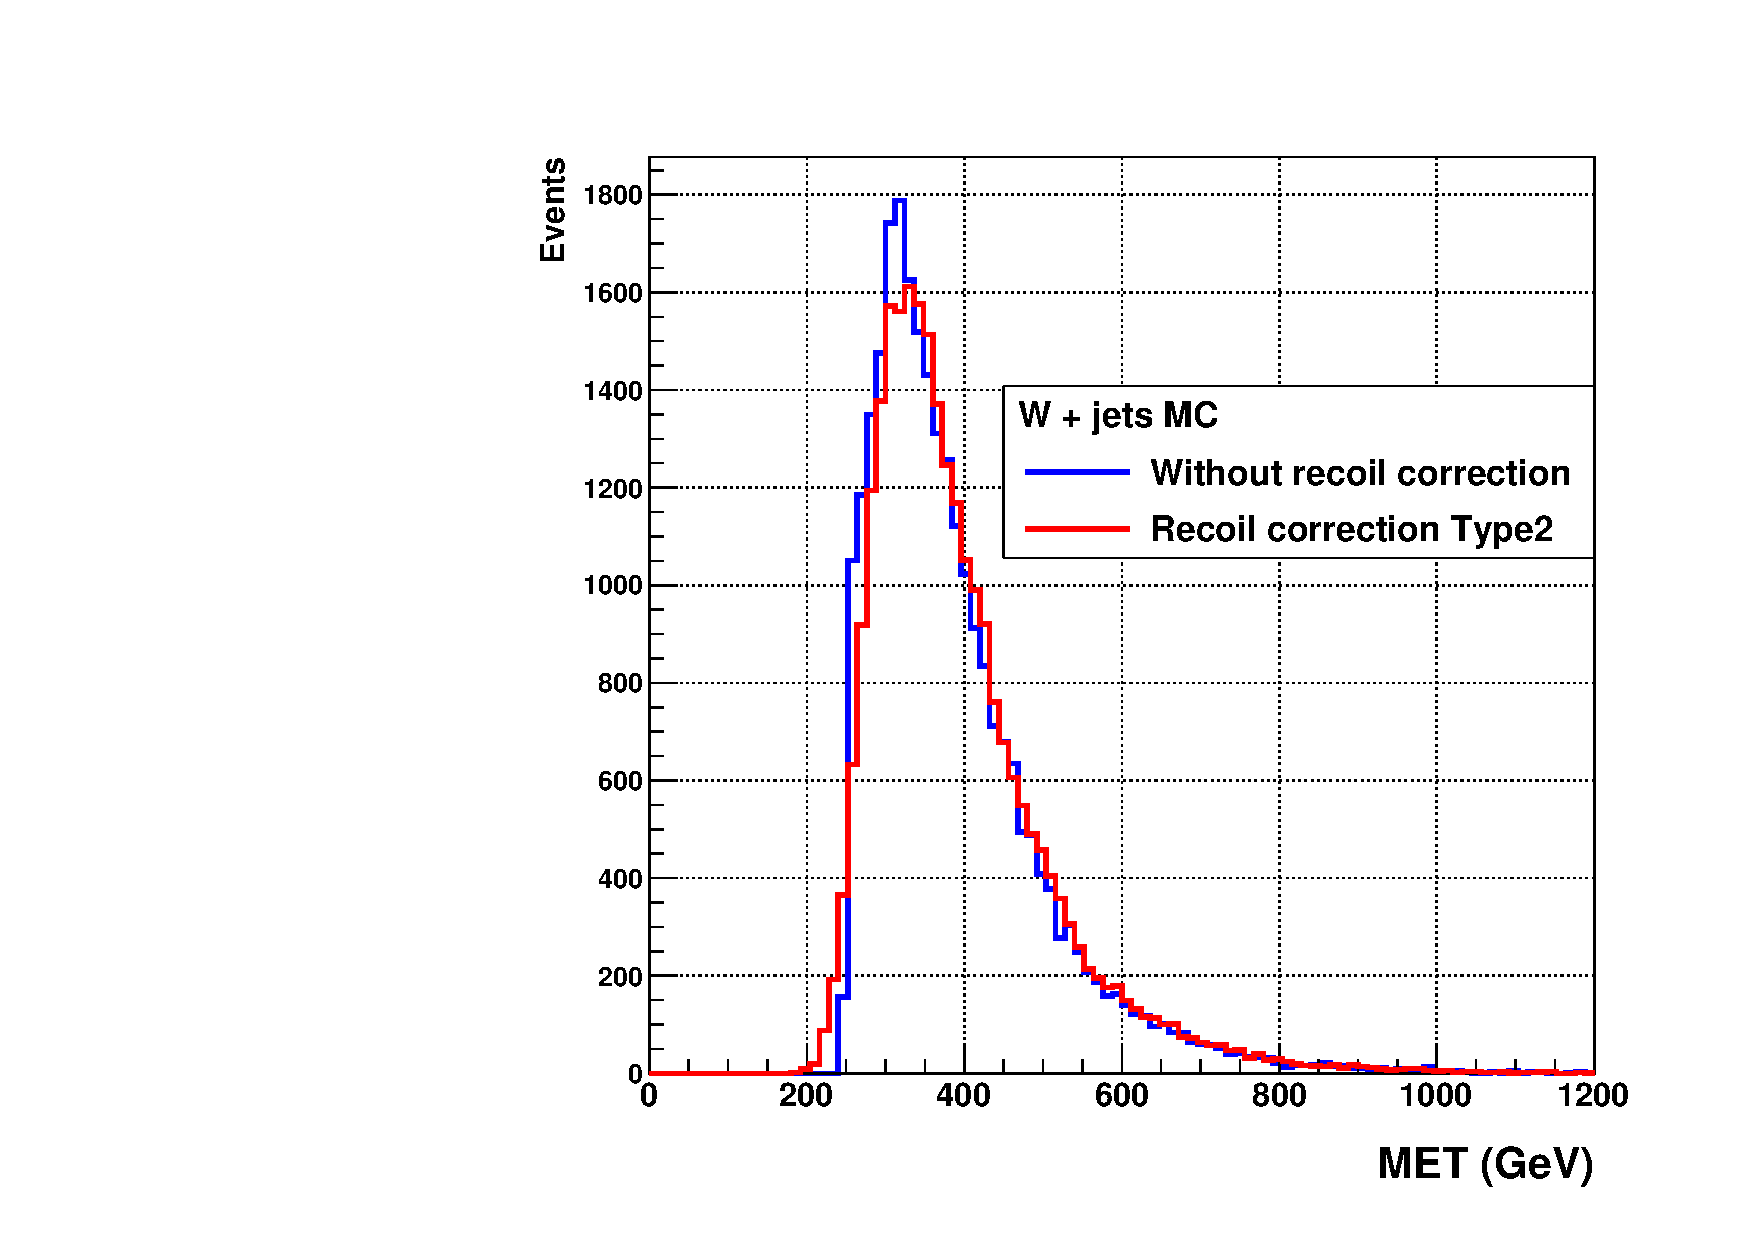
\includegraphics[width=230pt]{figuresARC/recoil/compRecoilCorrWjetsARC.pdf} &
  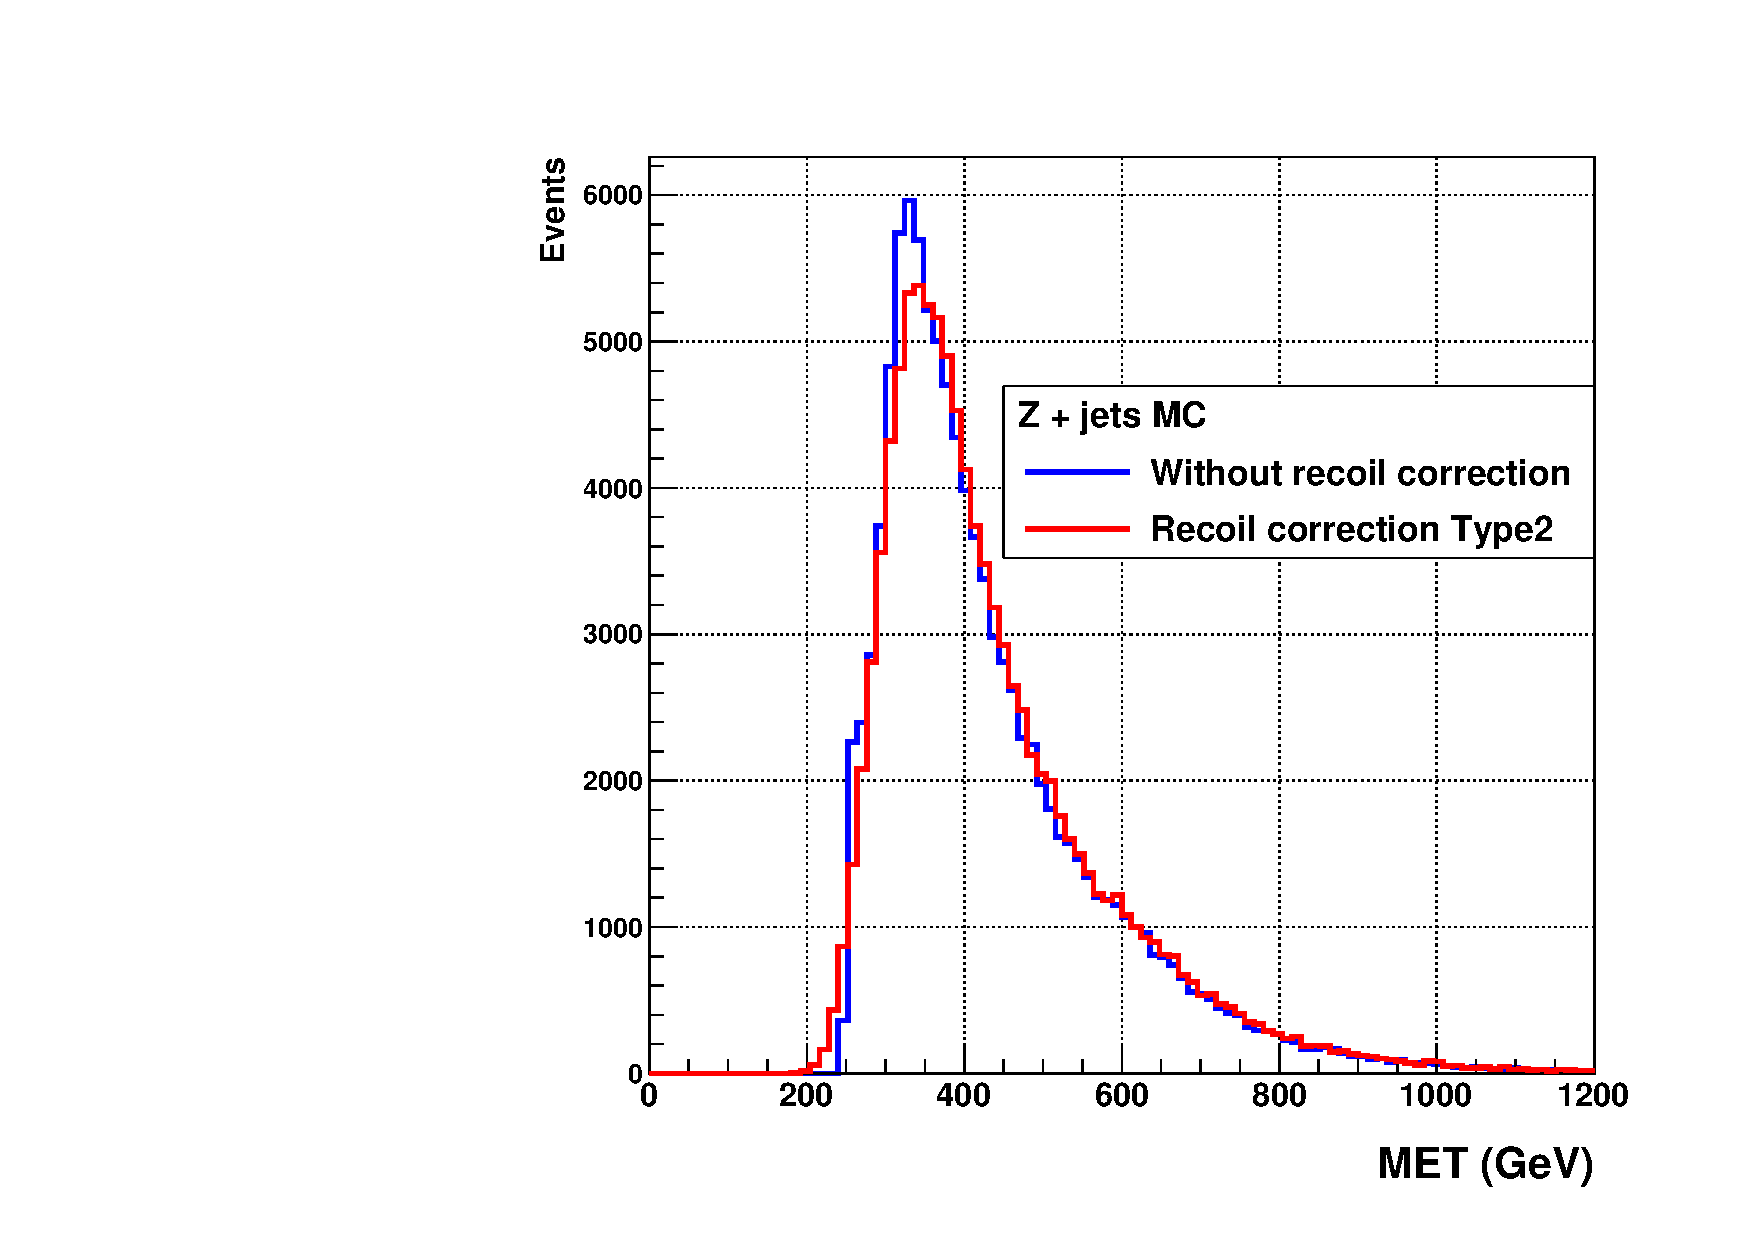
\includegraphics[width=230pt]{figuresARC/recoil/compRecoilCorrZjetsARC.pdf} \\
\end{tabular}
\label{fig:METrecoil}
\end{figure}




\section{Jets}\label{jets}

\par Jets are reconstructed using the PF technique. Charged hadrons not originating from the primary vertex are discarded in a process called ``charged hadron subtraction'' (CHS). The resulting list of particles are used as input to the anti-$\kt$ jet clusterging algorithm with a distance parameter $R$, implemented in the FastJet package. It is applied to the jets a technique based on jet areas that provides jet-by-jet corrections for pileup and underlying-event effects. Jet energies are further corrected using $\pt$ and $\eta$ dependent correction factors. These corrections are derived from MC simulation and are supplemented by residual corrections from dijet and photon+jet events in data. Figure \ref{fig:JEC} shows the comparison of the jet mass distributions before and after apply the JEC.

\begin{figure}[!ht]
\caption{Comparison between corrected and uncorrectd jets (JEC) for the jet mass distribution corresponding to a graviton signal sample  of 1 TeV ($X \rightarrow ZZ$). As it can be observed the corrected distribution shows a peak close to the Z mass (91 GeV).}
\begin{center}
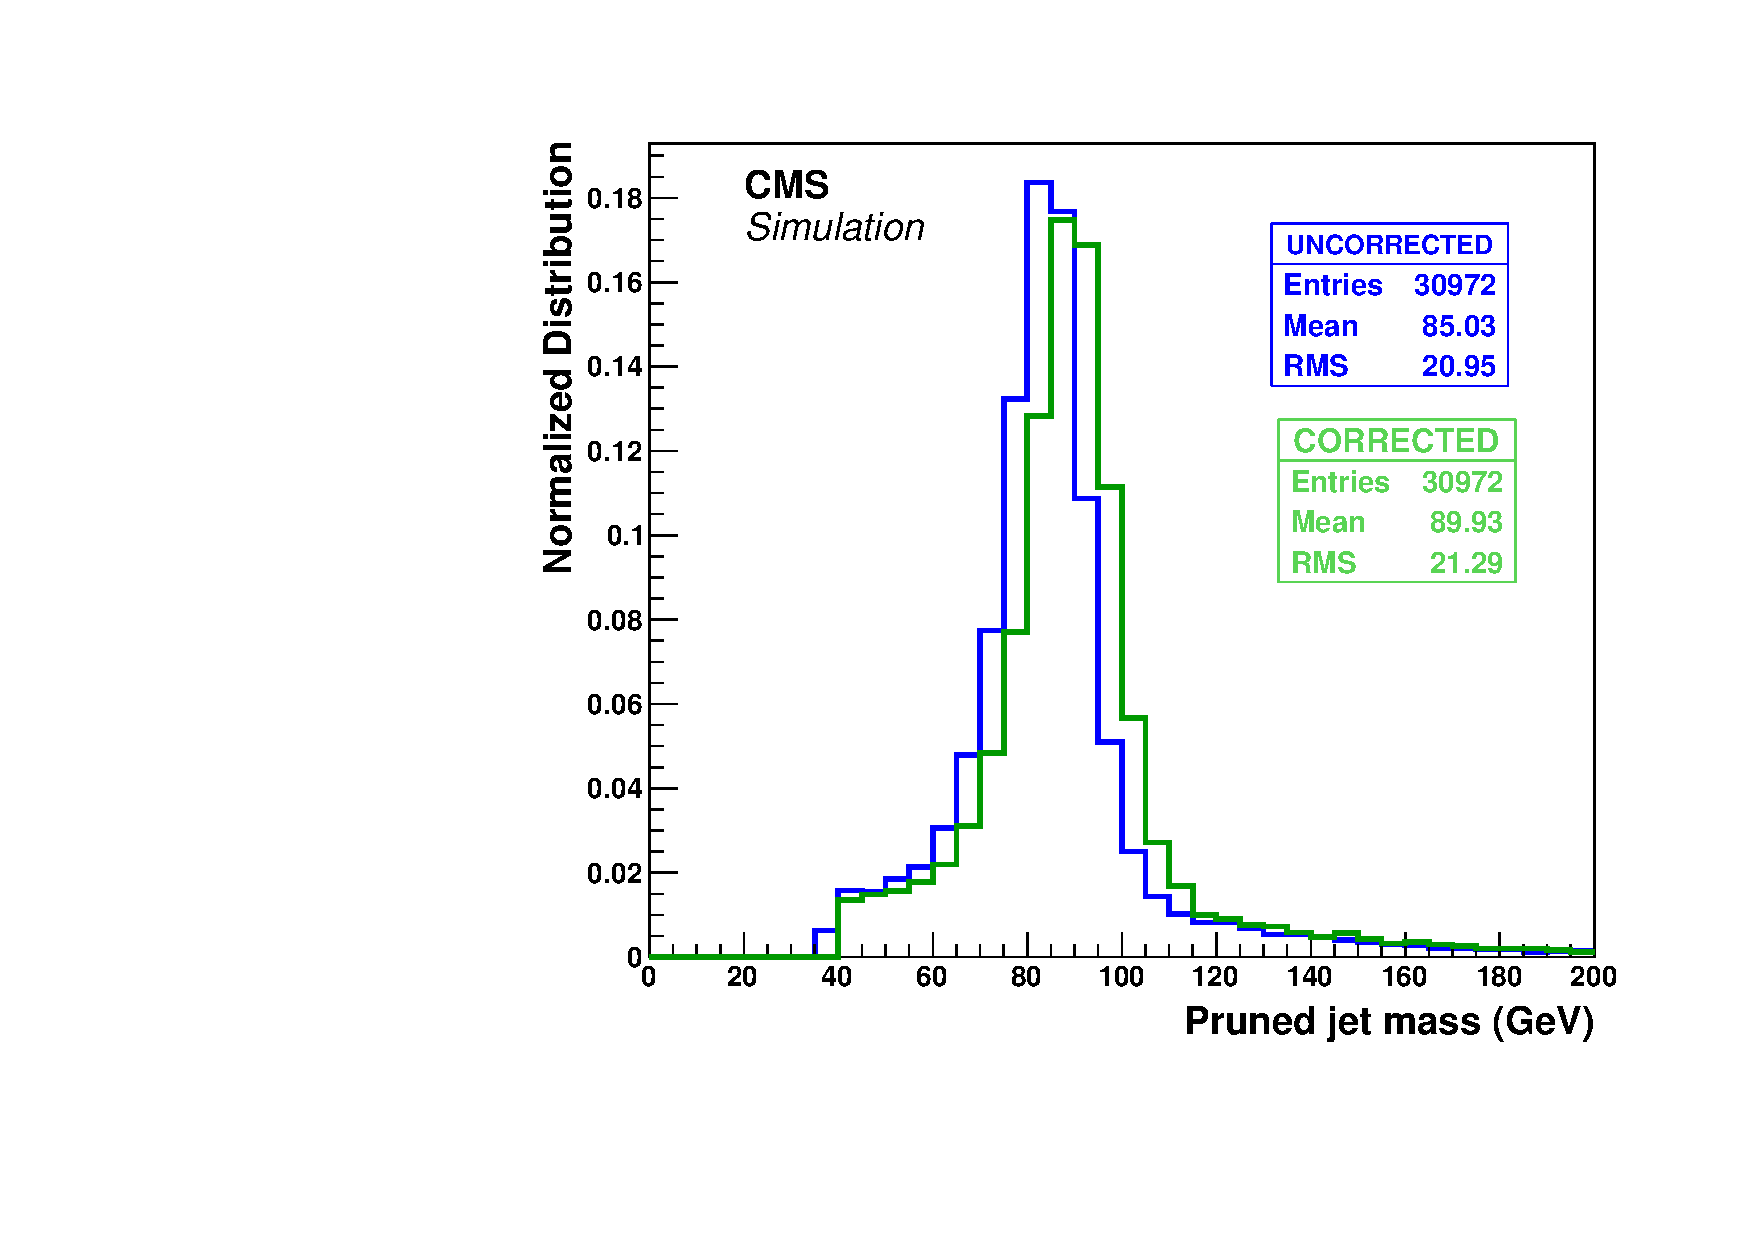
\includegraphics[width=250pt]{figures/Objects/jetcomparison.pdf}     
\end{center}
\label{fig:JEC}
\end{figure}

Loose jet identification criteria are applied to remove spurious jet-like features associated with calorimeter noise. To supress additional instrumental and beam-related backgrounds, events are rejected if less than 10$\%$ of the energy of the highest $\pt$ jet (leading jet) is carried by charged hadrons, or if more than 80$\%$ of this energy is carried by neutral hadrons.
Figure \ref{fig:jetclen} shows the charged hadron fraction (CHF) and neutral hadron fraction (NHF) distributions for events obtained with the full analysis selection after the cleaning cuts were applied. 

\begin{figure}[!ht]
\caption{Jet hadronic energy fractions after the cleaning cuts.}
\begin{tabular}{cc}
  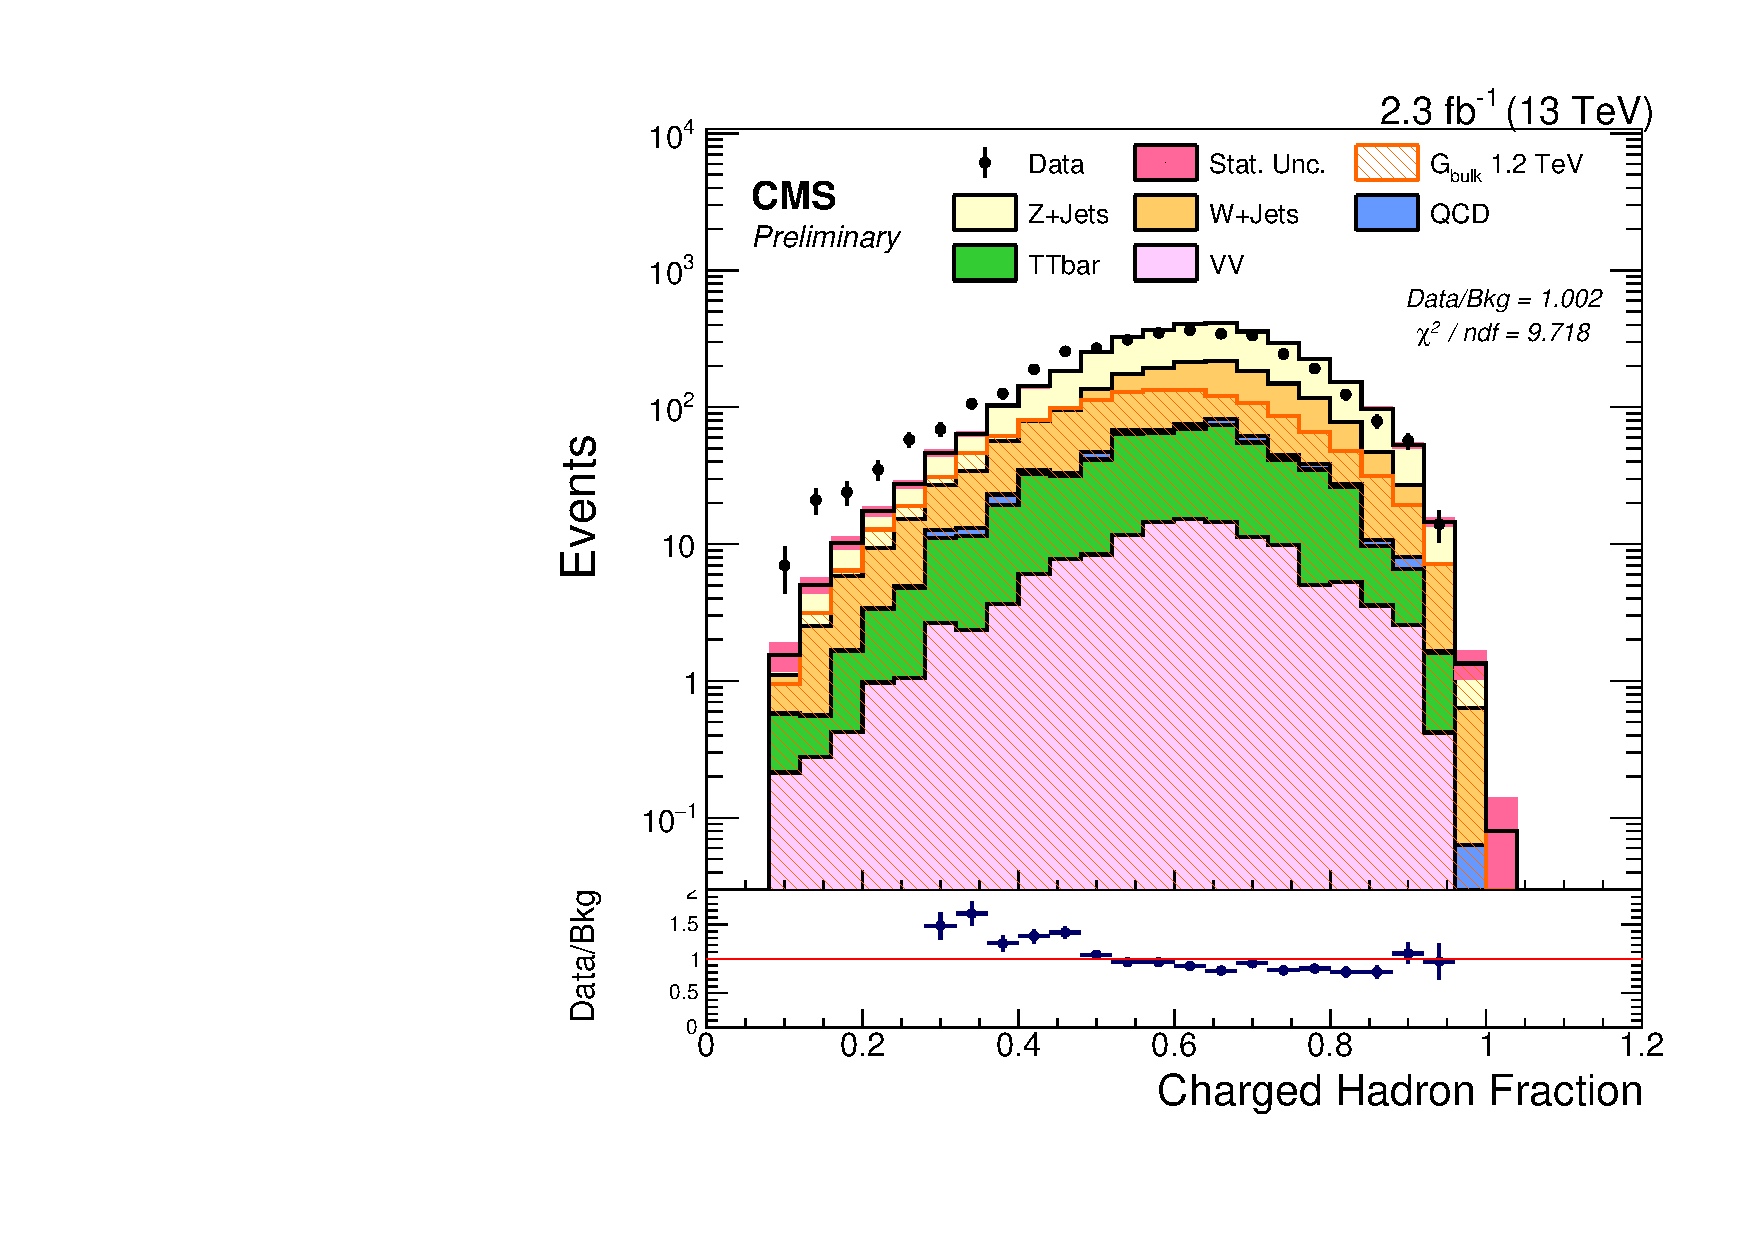
\includegraphics[width=230pt]{figuresCONDI/OBj/LOG_can_h_chf.pdf} &
  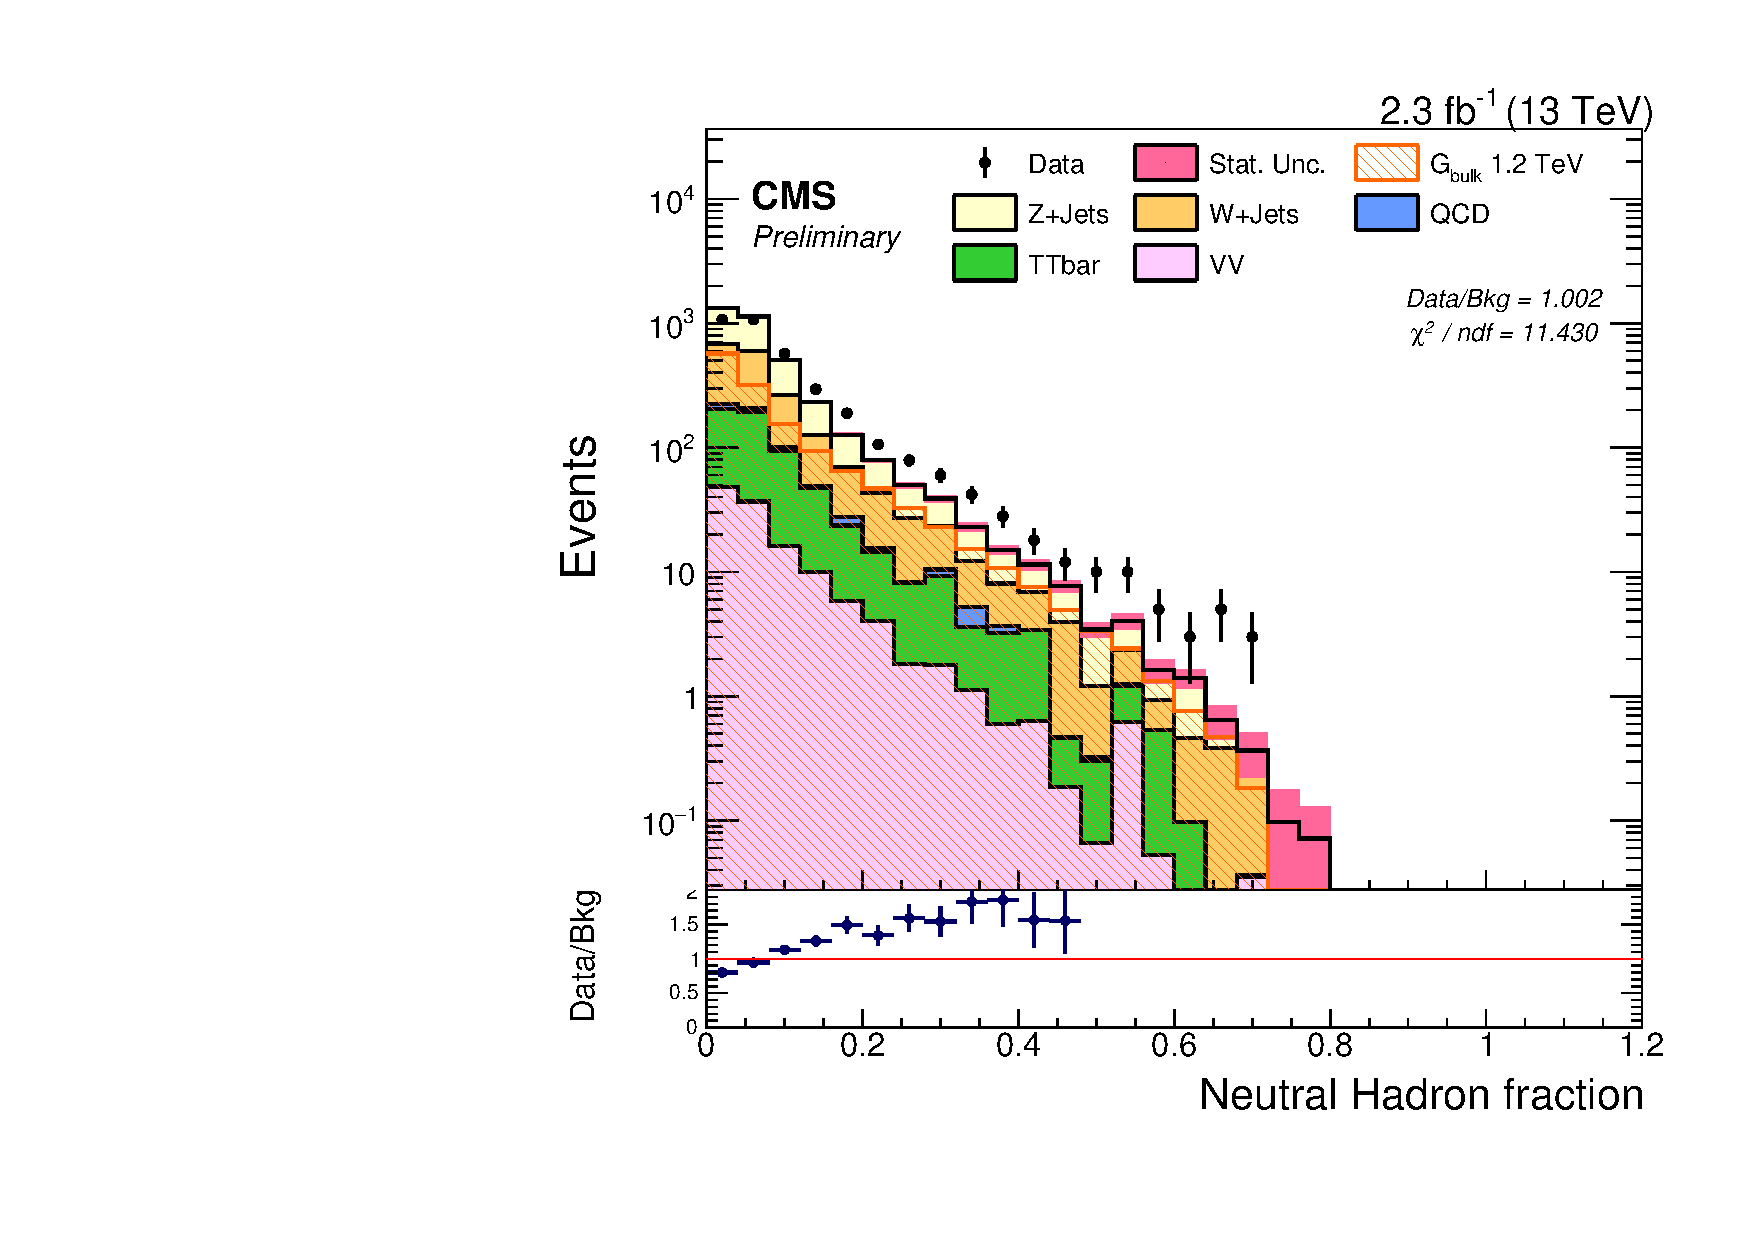
\includegraphics[width=230pt]{figuresCONDI/OBj/LOG_can_h_nhf.pdf} \\
\end{tabular}
\label{fig:jetclen}
\end{figure}

In addition jet energy resolution smearing factors reported in Table \ref{tab:JER},  were applied in the simulation aiming to improve the difference between Data and MC.

\begin{table}[!ht]
\begin{small}
\begin{center}
\caption{Jet energy resolution scaling factors and uncertainty.}
\label{tab:JER}
\begin{tabular}{cc} \hline
$\left| \eta \right|$ region  & Data/MC SF  \\ \hline
0.0-0.5 &  1.095 $\pm$ 0.018  \\
0.5-0.8  &  1.120 $\pm$ 0.028\\
0.8-1.1  &  1.097 $\pm$ 0.017 \\
1.1-1.3  &  1.103 $\pm$ 0.033 \\
1.3-1.7  &  1.118 $\pm$ 0.014 \\
1.7-1.9  &   1.100 $\pm$  0.033\\
1.9-2.1 &  1.162 $\pm$ 0.044   \\
2.1-2.3  &  1.160 $\pm$ 0.048 \\
2.3-2.5  &  1.161 $\pm$ 0.060 \\ 
2.5-2.8  &  1.209 $\pm$ 0.059  \\
2.8-3.0  &  1.564 $\pm$ 0.321  \\
3.0-3.2  &  1.384 $\pm$ 0.033  \\
3.2-5.0  &  1.216 $\pm$ 0.050  \\
\end{tabular}
\end{center}
\end{small}
\end{table}

To identify the hadronic decays of boosted V bosons, jets are clustered using the anti-$\kt$ algorithm with a distance parameter $R=0.8$ namely ``AK8 jets''. The leading AK8 jet is required to be inside the tracker acceptance ($\left| \eta\right| <$ 2.4.) and to have $\pt >$ 200 GeV.
The AK8 jet with the highest $\pt$ is associated to the $V \rightarrow q \bar{q}'$ candidate where the two quarks are merged to the same V-jet.
In addition, another collection of jets clustered with the anti-$\kt$ algorithm with a distance parameter $R=0.4$, called ``AK4 jets'', is used primarily for vetoing the presence of b-jets. The AK4 jets are required to have $\pt$ larger than 30 GeV and $\left| \eta\right| <  2.4$. Figure \ref{fig:ak4Multi} shows the ak4jets multiplicity in events that pass the final analysis selection.

\begin{figure}[!ht]
\caption{ak4Jets multiplicity.}
\begin{center}
  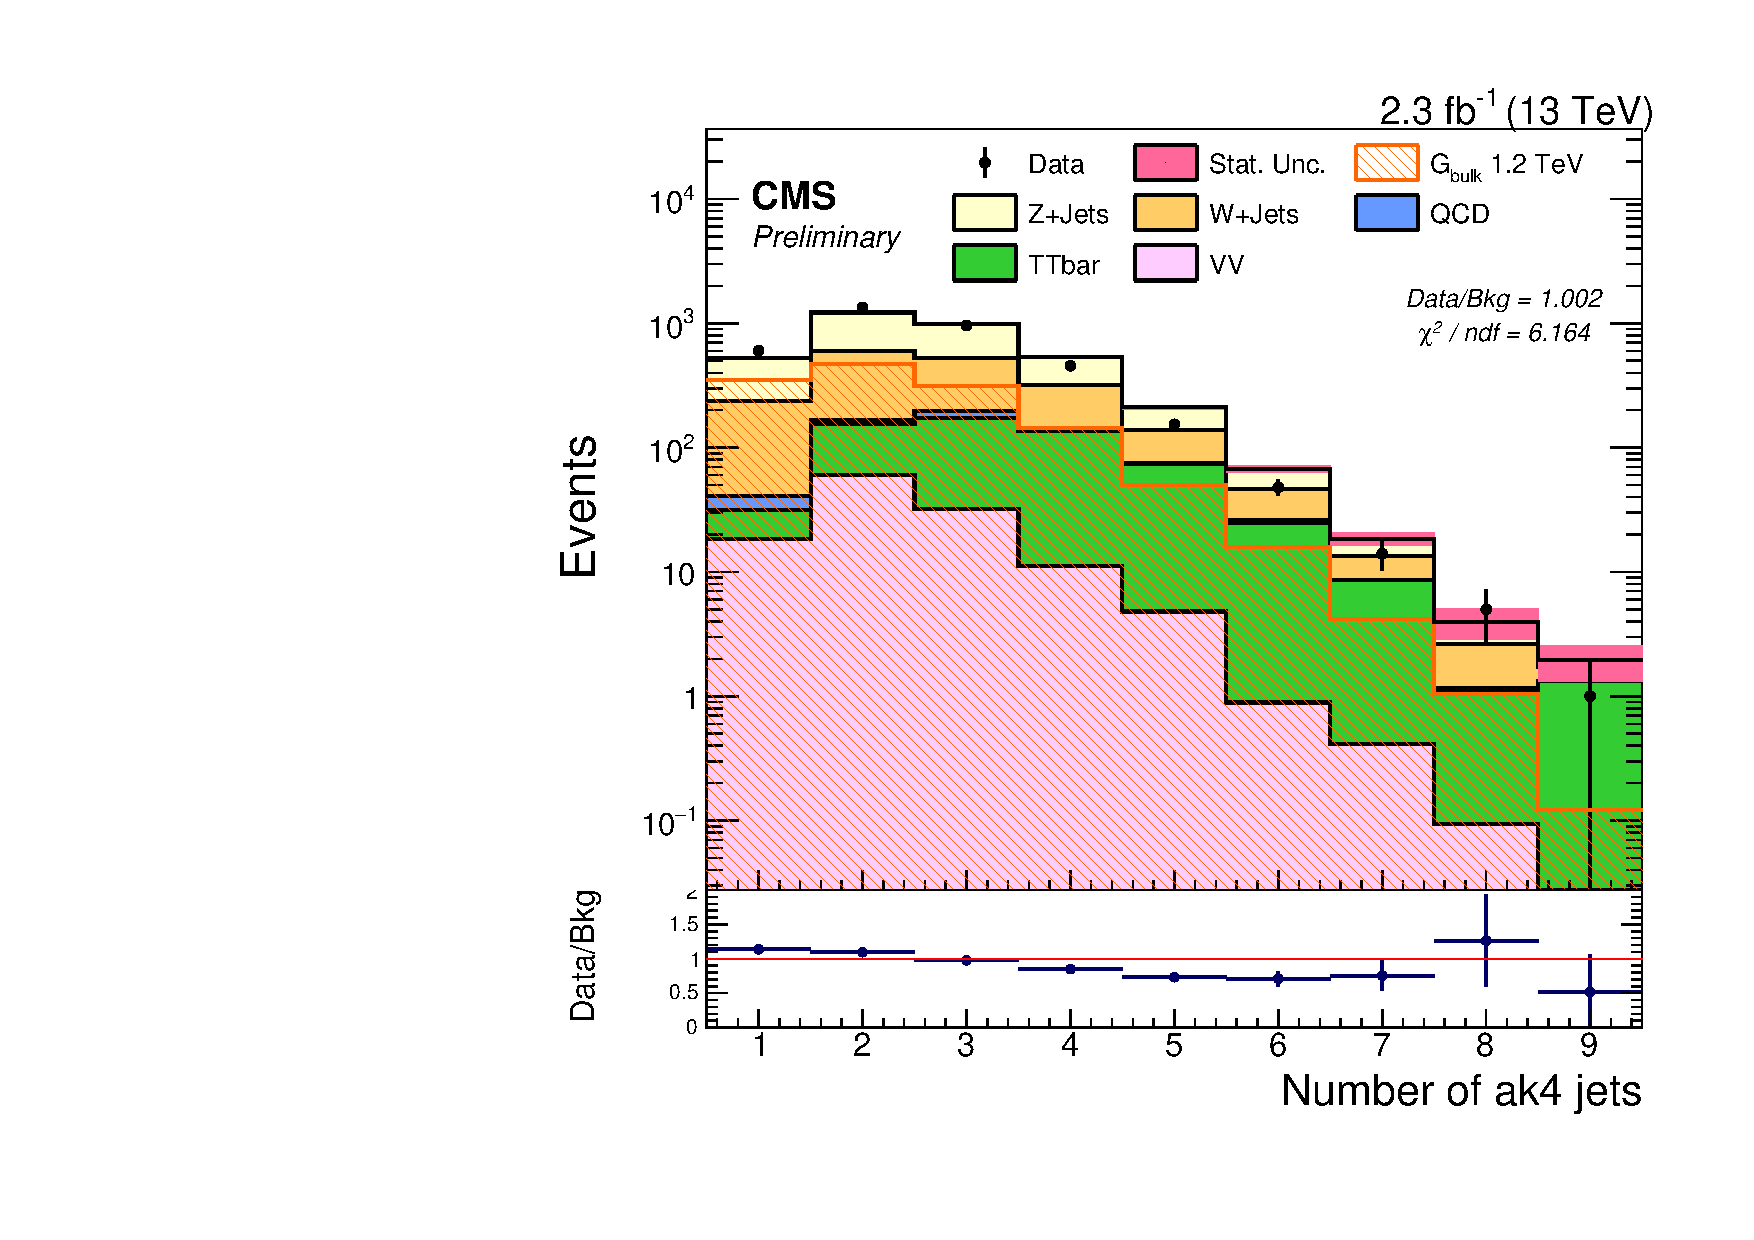
\includegraphics[width=250pt]{figuresCONDI/OBj/LOG_can_h_numjets.pdf}
\end{center}
\label{fig:ak4Multi}
\end{figure}

To identify b-jets, the medium working point of the inclusive combined secondary vertex b-tagging algorithm is applied to the reconstructed AK4 jets. We also required the b-jets to be spatially separated from the AK8 jets by at least $\Delta R = \sqrt{(\Delta \eta)^2+(\Delta \phi)^2}$ = 0.8, where $\Delta \eta$  and $\Delta \phi$ are differences between the b-jet and the AK8 jet directions in the pseudorapidity and the azimuthal angle. b-tagging Efficiency distributions in function of the  $\pt$ and $\left|\eta\right|$ of the jets were derived from simulation. The figure \ref{fig:bjetsscalefactor}  shows the efficiency maps for some MC samples, which are defined as 2D histograms with variable-sized bins in jet $\pt$ and $\left|\eta\right|$.
The ratio of the b-tagging efficiency between data and simulation is used as a scale factor to correct  $t\bar{t}$, V+jets, and signal simulated events.

\begin{figure}[!ht]
\caption{Derived efficiency maps for b-tagging in function of the $\pt$ and $\left|\eta\right|$ of the jet in MC samples (left) $t\bar{t}$ sample  (right) Z +jets sample, for jets with flavor b.}
\begin{tabular}{cc}
  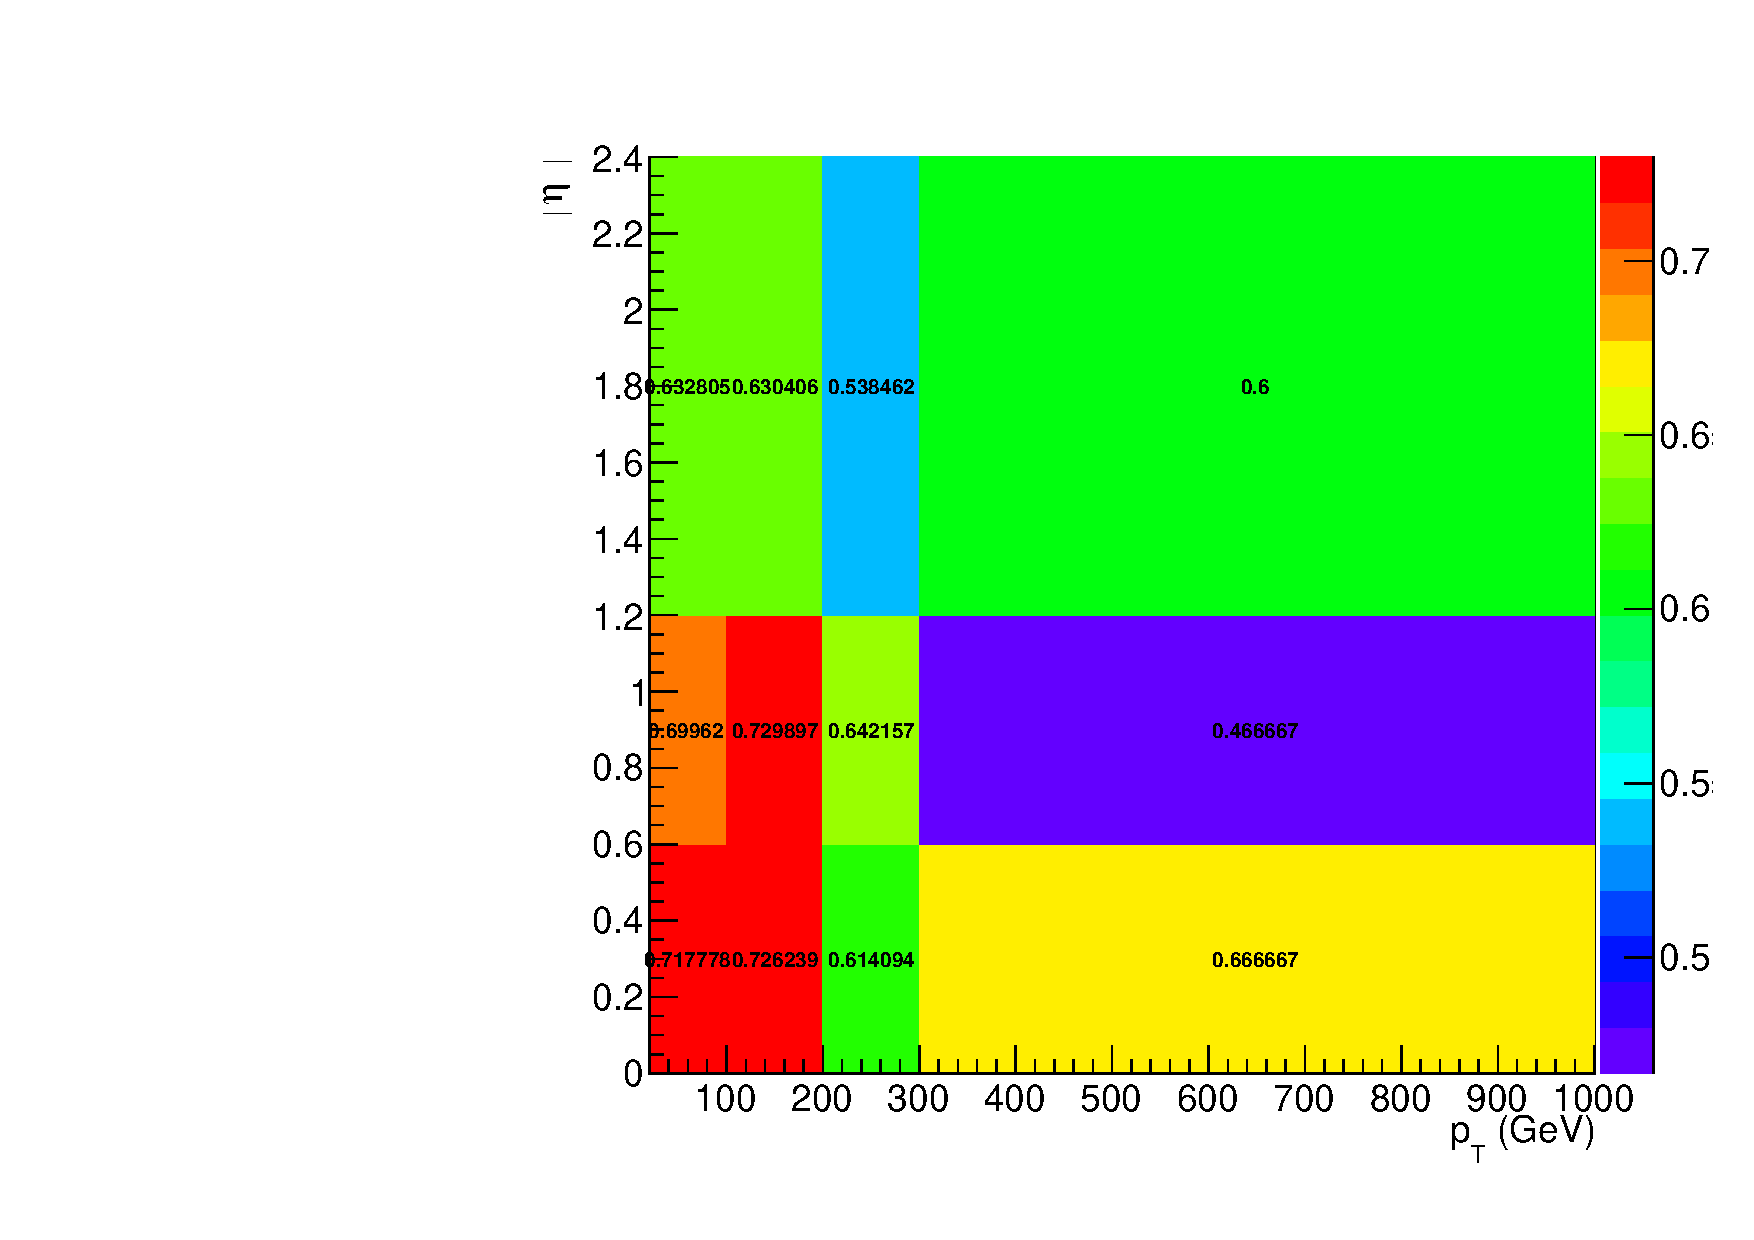
\includegraphics[width=200pt]{figures/SFbtagg/effmapTT.pdf} &
  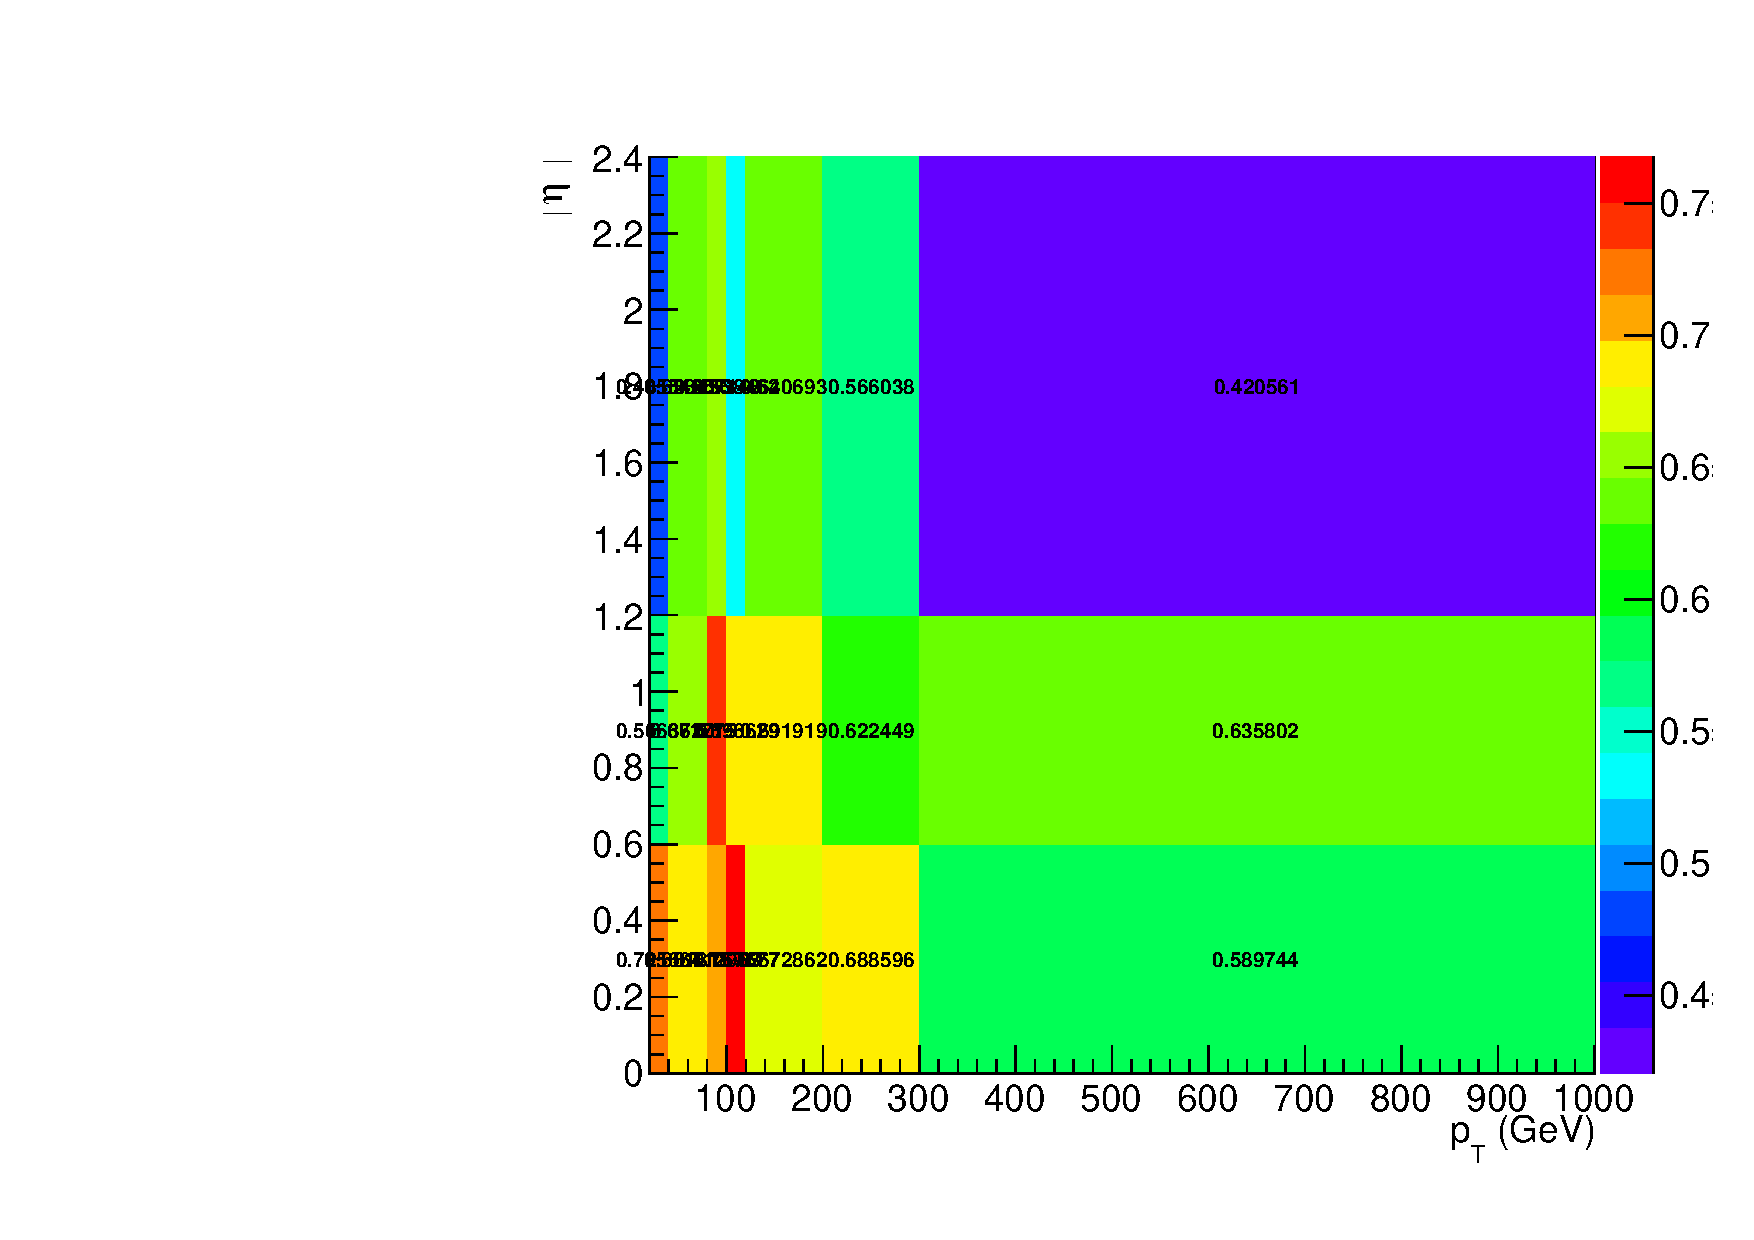
\includegraphics[width=200pt]{figures/SFbtagg/effmapZJ.pdf}\\
\end{tabular}
\label{fig:bjetsscalefactor}
\end{figure}


\section{Hadronic V identification using jet substructure}
\label{sec:HadronicVid}

\par The decay of heavy resonances in dibosons $X \rightarrow VZ$ produce objects with very high $\pt$. When the boost of the V-boson is large enough i.e. $\pt>$200 GeV, the final state hadrons from the decay $V \rightarrow q\bar{q}'$  merge into a single jet. In those cases, the traditional techniques relying on resolved jets are no longer applicable. However, jet substructure methods can be used to identify those jets arising from decays of W, Z or H bosons.
In this analysis, a ``V-tagging" technique based on two jet subtructure methods, pruning  and N-subjettiness, is used in order to discriminate between jets arising from V-decays and those from QCD backgrounds.

\par The leading AK8 jet in the event is considered a V-jet candidate if its pruned mass ($m_{\text{jet}}$), computed from the sum of the four-momenta of the constituents surviving the pruning, falls in the range $65\leq  m_{\text{jet}} \leq105$ GeV. Jets coming from hadronic V decays in signal events are characterized by lower values of $\tau_{21}$  compared to the SM background. To optimize the analysis sensitivity, we distinguish two samples of data:
\begin{itemize}
\item
High Purity (HP) :  $\tau_{21}< 0.45$
\item
Low Purity (LP)  : $0.45 < \tau_{21} < 0.75$
\end{itemize}

Events with $\tau_{21} > 0.75$  are rejected due to very low signal efficiency.
The combined use of the pruned mass and the $\tau_{21}$ allows us to do the V-tagging of a jet with different degrees of purity.
The $\pt$ and $\tau_{21}$ distributions of the highest AK8 jet in the event for data, SM backgrounds, and a bulk graviton
signal sample are shown in Fig. \ref{fig:Vtagg}  after applying a $65\leq  m_{\text{jet}} \leq105$ GeV requirement.
The distribution of $\tau_{21}$  shows some disagreement between data and simulation which is due primarily to a mismodeling of the parton showering \cite{CMS-PAS-EXO-12-021}.

\begin{figure}[!ht]
\caption{ Distribution of $\pt$ (left) and $\tau_{21}$ (right) for the leading AK8 jet in events passing the
final selection in the pruned jet mass signal region for data, SM backgrounds and for a bulk graviton signal sample (1.2 TeV resonance mass and $\tilde{k}$ = 0.5).}
\begin{tabular}{cc}
  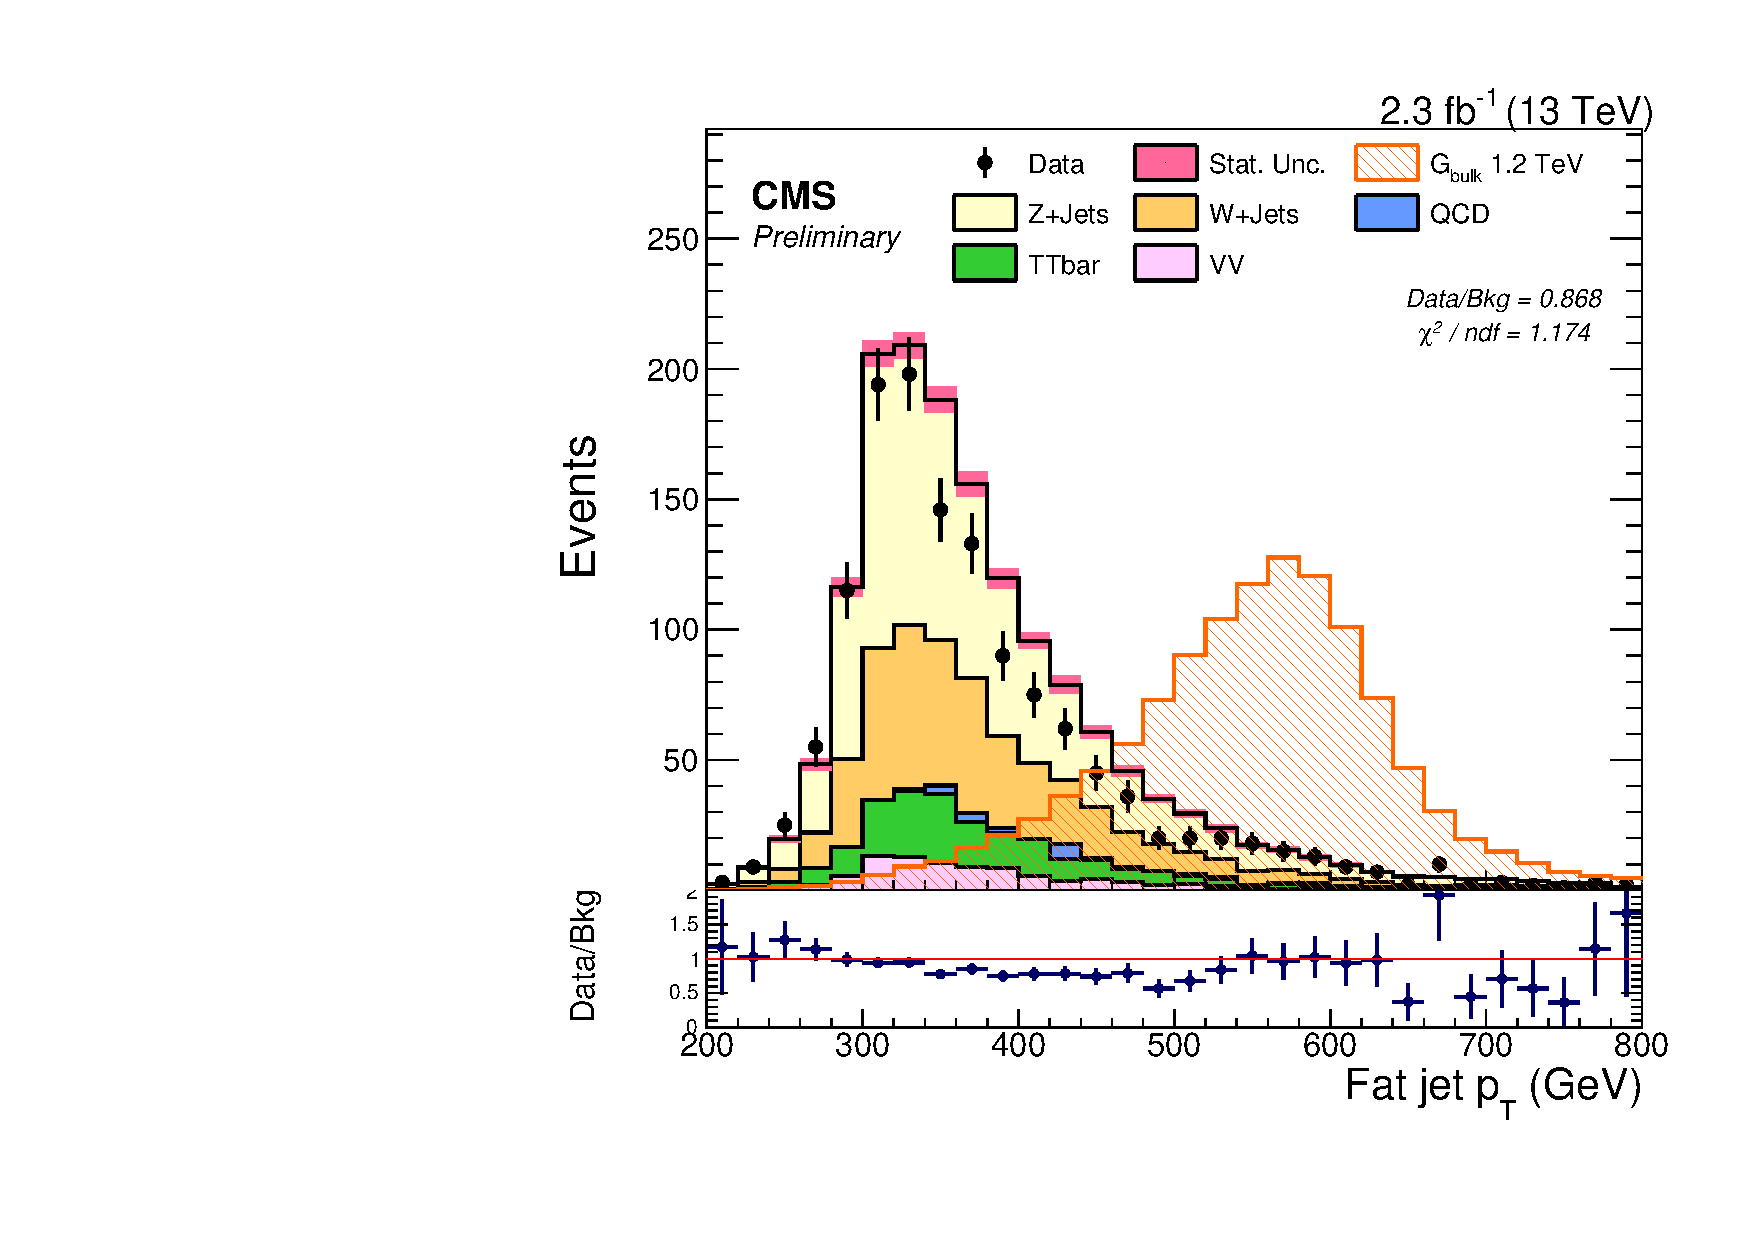
\includegraphics[width=230pt]{figures/can_h_ptZjj.pdf} &
  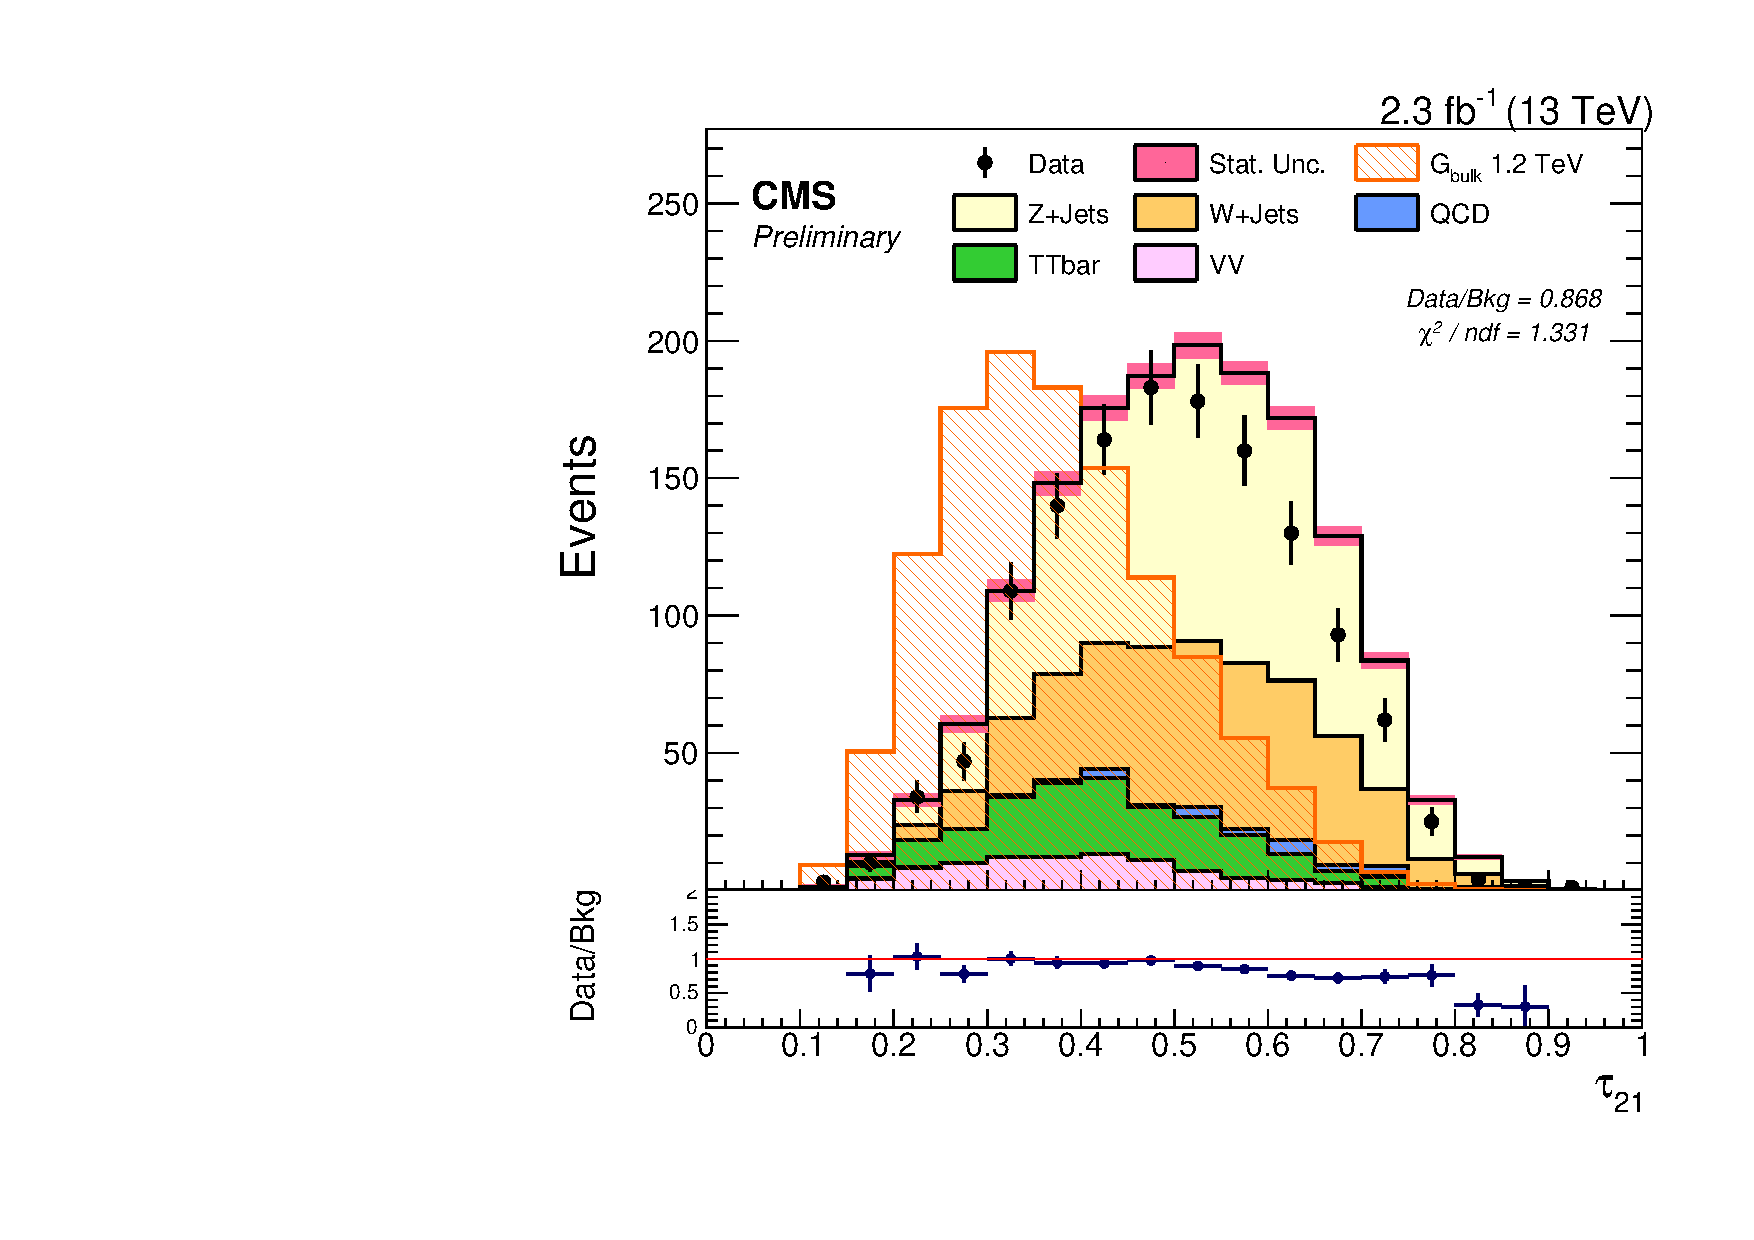
\includegraphics[width=230pt]{figures/can_h_tau21.pdf}\\
\end{tabular}
\label{fig:Vtagg}
\end{figure}

The discrepancies between data and simulation in the jet substructure variables $m_{\text{jet}}$ and $\tau_{21}$ are corrected using scale factors for V-tagging efficiency.
A sample of high-$\pt$ W bosons, which decay hadronically and are reconstructed as a single AK8 jet, was studied in $t\bar{t}$ and single top-quark events. Scale factors for the $\tau_{21}$ selection efficiency are extracted following the method described in Ref. \cite{Khachatryan2014aa}. A simultaneous fit to the jet mass distributions, in both data and simulation, before and after the $m_{\text{jet}}$ and $\tau_{21}$ requirements, is performed to separate the W-signal from the combinatorial components in the top-enriched sample. The fit results are used to extract data-to-simulation efficiency scale factors to identify an isolated hadronic W boson. The scale factors are reported in Table \ref{tab:VtaggSF} and are used to correct the total signal efficiency. The uncertainty on those scale factors is then assigned as systematic uncertainty of the method.

\begin{table}[h!]
 \centering
  \caption{Scale factors for the $\tau_{21}$ efficiency selection derived from data and simulation in a top-quark enriched sample.}
  \label{tab:VtaggSF}
  \begin{tabular}{cc}
\hline
$\tau_{21}$ Selection                 &          Efficiency scale factor          \\
\hline
$\tau_{21} < 0.45$                    &          $0.942 \pm 0.063$                  \\
$0.45 < \tau_{21} < 0.75$             &          $1.268 \pm 0.332$                   \\
\hline
\end{tabular}
\end{table}



\section{Muons}

Muons candidates are reconstructed by associating track measurements in the inner tracker and in the muon system. A set of requirements based on the impact parameter of the track and on the number of hits recorded in the silicon tracker and in the muon chambers have to be fulfilled in order to identify loose muons(referencia). The resulting muons are required to have $\pt > 10$ GeV and $\left| \eta\right| <$ 2.4. To reject nonprompt or misidentified leptons, requirements are imposed on the isolation criteria, based on the sum of deposited energies. The relative isolation parameter (RelIso) is defined as the contributions from the total transverse momentum of all charged hadrons, the transverse energies ($\ET$)  of all photons, and the $\ET$ of all neutral hadrons reconstructed by the PF algorithm within a cone of radius $\Delta R < 0.4$ centered on the muon  track direction, divided by the muon track $\pt$. Identified muons with RelIso values below 0.25 are considered isolated and used in the analysis. Table \ref{tab:MuonID} summarize the criteria used to identify muons.

\begin{table}[h!]
 \centering
  \caption{Muon identification criteria.}
  \label{tab:MuonID}
  \begin{tabular}{|c|p{15cm}| }
\hline
Variable                 &          Criteria          \\
\hline
ID                    &          Loose muon : particle identified as a muon by the Particle-Flow event reconstruction, and that is also reconstructed either as a global-muon or as an arbitrated tracker-muon.    \\ \hline
Isolation             &          PF-based combined relative isolation (RelIso) with $\Delta \beta$ correction, less than 0.25                   \\
\hline
\end{tabular}
\end{table}

In order to reduce electroweak backgrounds (W+jets), we reject events that contain identified muons. Some scale factors (SF) was derived centrally to improve the agreement between data and MC due to identification and Isolation of the muons. We use the SF to reweight the events that contain muons in the following way:
First we define a weight called \emph{muonWeight},  which is equal to 1 for the events that do not contain muons. For the events that contains muons the weight will be:
\begin{eqnarray}
\text{muonWeight} = 1-\text{SF}
\end{eqnarray}
As the SFs are numbers close to 1, the possible outcomes will be:
\begin{itemize}
\item
if SF $<1$ then the muonWeight gives a small positive number
\item
if SF  $=1$ then the muonWeight = 0 (is like apply the veto)
\item
if SF $>1$ then the  muonWeight gives a small negative number
\end{itemize}
We use the equivalence ( muonWeight = 1 $\equiv$ No veto in the event) and (muonWeight = 0 $\equiv$ veto the event)

An association between the reconstructed and the generated muons was performed using a geometrical matching with a cone of $\Delta R(\text{recoMuon},\text{genMuon}) = 0.1$. To resolve ambiguities in the matching, among all the possible combinations, we choose the minimum $\Delta R$ in the calculation. In the figure \ref{fig:Match} we show the minimum $\Delta R$ between the reconstructed and generated muons for a MC signal sample of 1 TeV after apply the final selection of the analysis. The application of the SF is base on kinematic information ($\pt$,$\eta$) of the reconstructed muons that pass the MC matching, taking in account the generator level information of the muons in this process.

\begin{figure}[!ht]
\caption{Minimum $\Delta R$ between reconstructed and generated muons for a signal mass point of 1 TeV.}
\begin{center}
  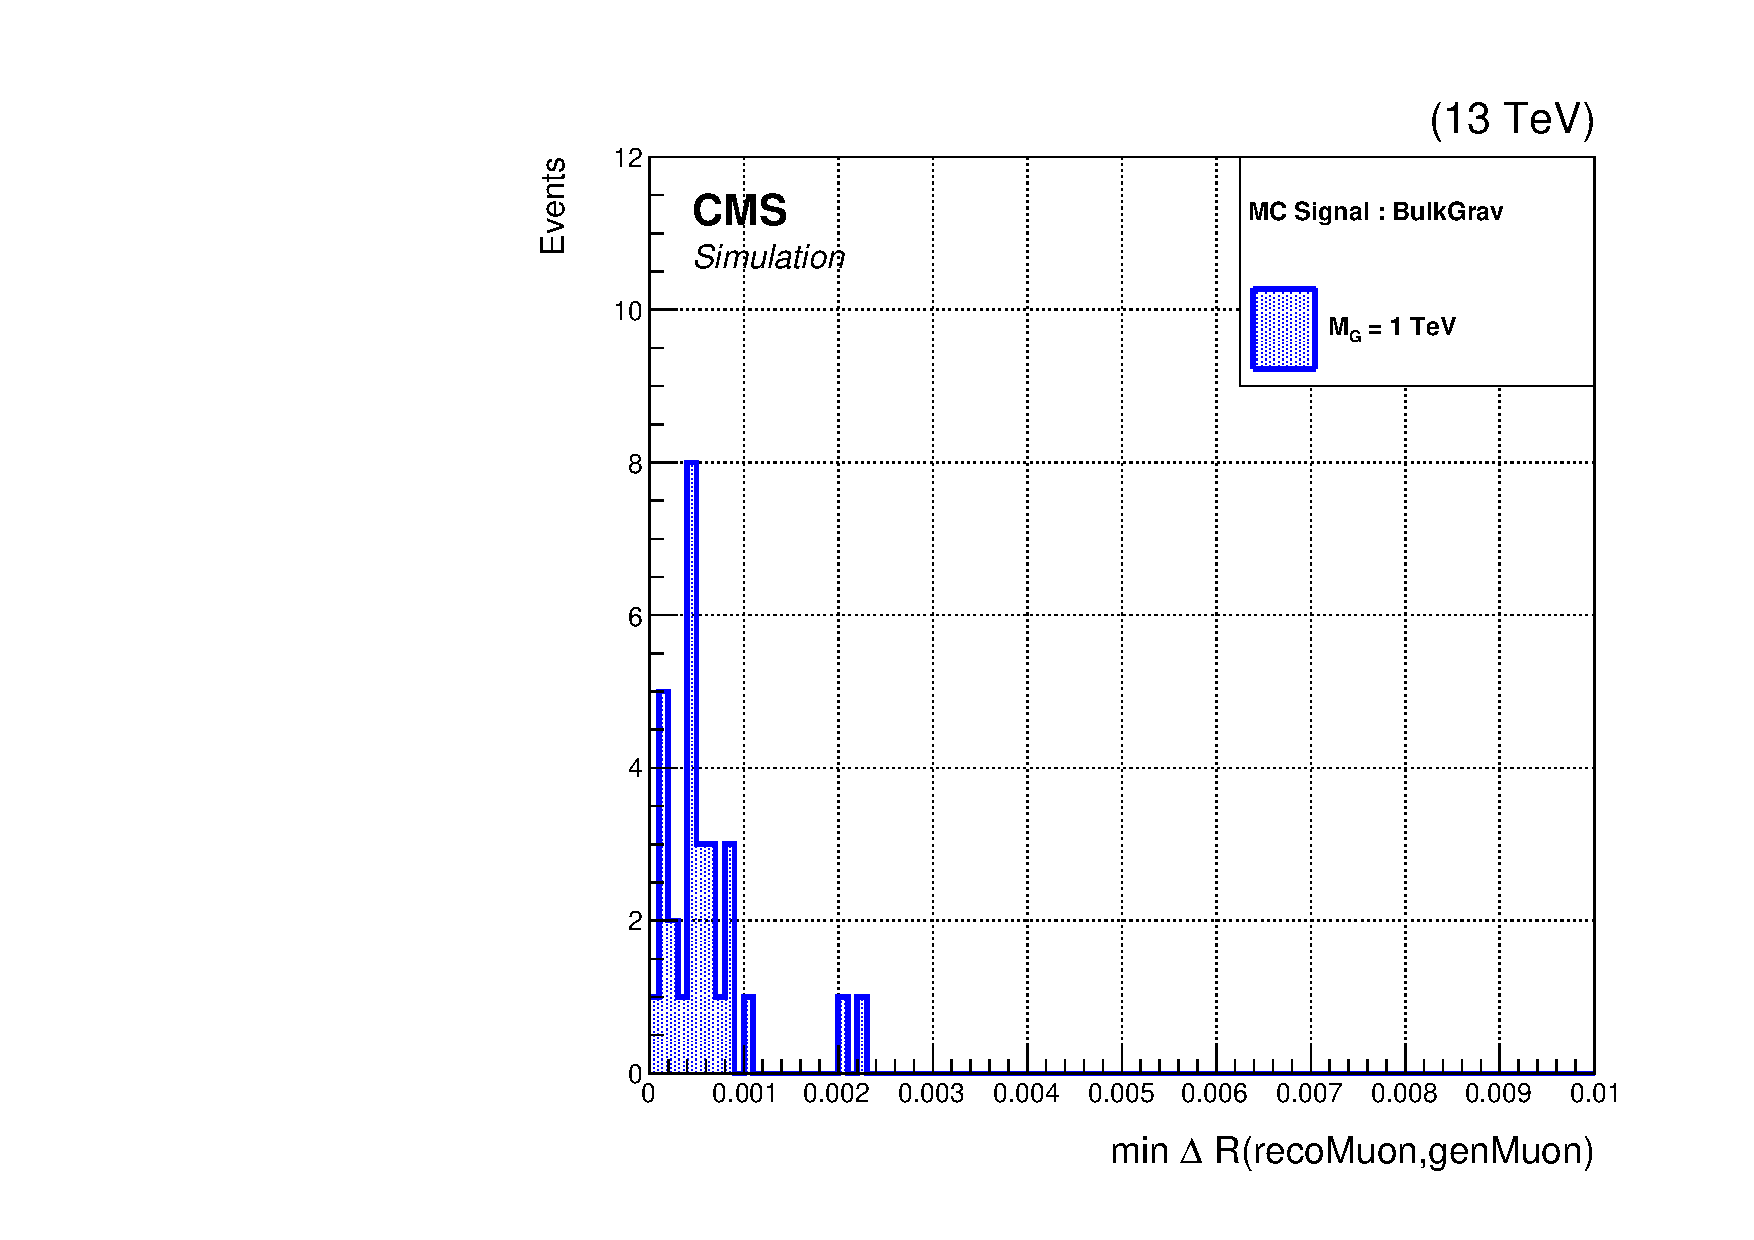
\includegraphics[width=250pt]{figuresCONDI/OBj/matchingmuons.pdf} 
\end{center}
\label{fig:Match}
\end{figure}

\section{Electrons}

Electrons candidates are reconstructed by associating a charged particle track with an ECAL supercluster, including energy depositions from final-state radiation. The resulting electron candidates are required to have $\pt > 10$ GeV, $\left| \eta\right| <$ 2.4, and to satisfy identification criteria designed to remove photon conversions, jets misidentified as electrons, and electrons from semileptonic decays of bottom and charm quarks. Identified electrons with RelIso values below 0.1 are considered isolated and used in the analysis. Events with identified electrons are vetoed to reduce W+jets background. SFs were derived centrally to improve the agreement between data and MC due to identification and Isolation of the electrons. A MC matching was implemented in the reconstructed electrons aiming to applying the SF taking in account the generator level information of the electrons. The method to apply the SFs over the MC samples to reweight the event was explained in the muons section.


\section{Taus}

The hadronic tau ($\tau_{h}$) decays are reconstructed and identified using the hadrons-plus-strips (HPS) algorithm. The algorithm is designed to reconstruct individual decay modes of the tau lepton, taking advantage of the PF algorithm. It also discriminate $\tau_{h}$ decays from quark and gluon jets, and from electrons and muons. In addition, tau-isolation requirements complement the identification process. Identified taus are required to have $\pt > 20$ GeV and $\left| \eta\right| <$ 2.3 to be used in the analysis.
Events with identified taus are removed in order to disminished W+jets background. We consider for the tau ID efficiency, the ratio between data and MC equal to 1, with an uncertainty of 6$\%$. This recommendation is valid for all isolation discriminators, $\pt$ and $\eta$ range, in Run-2 analyses. 


\section{Photons}\label{photons}

Photons candidates are reconstructed by clustering spatially correlated energy deposits in the ECAL. Photon identification is based on two main categories of observables: shower-shape and isolation variables which help to discriminate among signal photons and photons that arise from neutral mesons produced in jets or electrons misidentified as photons. Identified photons are required to have $\pt > 15$ GeV and $\left| \eta\right| <$ 2.5 to be used in the analysis. In order to reduce Z +$\gamma$ +jets and W + $\gamma$ +jets backgrounds  we reject events that contain photons.
Photons candidates are required to have a minimum $\pt$ of 15 GeV and $\left| \eta\right| < $2.5.
With the objective to identify photons we use a loose cut-based working point identification.
SFs were derived centrally to improve the agreement between data and MC due to identification and Isolation of the photons. We apply properly those scale factor over the MC samples to reweight the event as was explained in the muons section.

\section{Transverse mass}\label{MT}
The hadronic V-boson candidate ($V \rightarrow q \bar{q}'$) is reconstructed from the AK8 jet with the highest $\pt$. Due to the invisible decay of the Z boson ($Z \rightarrow \nu \bar{\nu}$), the reconstruction of the resonance mass is not directly viable and its total momentum can be constrained only in the plane transverse to the beam direction. Therefore, we will use as the final discriminant a quantity called ``transverse mass'', defined by
\begin{eqnarray*}
M_{VZ}^{T} = \sqrt{2 p_{T} \MET \left( 1-\cos(\Delta \phi)\right)}
\end{eqnarray*}
where $p_{T}$ is the transverse momentum of the AK8 Jet and $\Delta \phi$ is the angle between the jet $\pt$ and the $\MET$ vector.
